\chapter{Vulnerability}
\label{chap:vulnerability}
These vulnerability functions can be used directly by the Scenario Risk, Classical PSHA-based Risk and Probabilistic Event-based Risk calculators of the OpenQuake-engine (\cite{SilvaEtAl2014a}; \cite{PaganiEtAl2014a}). \\

A vulnerability model can be derived directly from loss data (either analytically generated or based on past seismic events), or by combining a set of fragility functions with a consequence model (see Section \ref{subsec:cons_model}). In this process, the fractions of buildings in each damage state are multiplied by the associated damage ratio (from the consequence model), in order to obtain a distribution of loss ratio for each intensity measure type. Currently only the latter approach is implemented in the Risk Modellers Toolkit, though the former method will be included in a future release.\\

The location of the consequence model must be defined using the parameter \verb=cons_model_file=, and load it into the Risk Modellers Toolkit using the function \verb=read_consequence_model=. The intensity measure levels for which the distribution of loss ratio will be calculated must be defined using the variable \verb=imls=.\\

The Risk Modellers Toolkit allows the propagation of the uncertainty in the consequence model to the vulnerability function. Thus, instead of just providing a single loss ratio per intensity measure type, it is possible to define a probabilistic model (following a \verb=lognormal= or \verb=beta= functions) or a non-parametric model (i.e. probability mass function - \verb=PMF=). This model must be defined using the variable \verb= distribution_type=.\\

The derivation of the vulnerability function also requires the previously computed \verb=fragility_model=. The function that calculates this result is contained in the module \verb=utils=. An example of this process is depicted below.

\begin{Verbatim}[frame=single, commandchars=\\\{\}, samepage=true]
cons_model_file = '../../../../../../rmtk_data/cons_model.csv'
cons_model = utils.read_consequence_model(cons_model_file)
imls = [0.1,0.2,0.3,0.4,0.5,0.6,0.8,0.9,1.0]
distribution_type = 'PMF'
vul_model = utils.convert_fragility_vulnerability(fragility_model,...
cons_model,imls,type_distribution)
\end{Verbatim}

The resulting vulnerability function can be saved using the function \verb=save_vulnerability=. This feature can export the vulnerability function using the OpenQuake-engine format (\verb=nrml=), or following a \verb=csv= format. Similarly to what was described for the fragility models, this indication should be provided using the variable \verb=output_type=. It is also possible to plot vulnerability functions, using the function \verb=plot_vulnerability_model=. In order to use these functions, it is necessary to import the module \verb=utils=. This process is demonstrated below.

\begin{Verbatim}[frame=single, commandchars=\\\{\}, samepage=true]
output_type = 'nrml'
utils.save_vulnerability(taxonomy,vulnerability_model,output_type)
utils.plot_vulnerability_model(vulnerability_model)
\end{Verbatim}

A detailed description of the \verb=nrml= format for vulnerability functions can be found on the OpenQuake-engine manual \citep{GEM2015}. For what concerns the structure of the \verb=csv= file, this format varies depending on how the uncertainty is being defined: parametric (lognormal or beta) or non-parametric (probability mass function). For the former case, an example is provided in Table \ref{table:vf_cont_csv}. The first row contains the building \verb=taxonomy=, the intensity measure type (\verb=IMT=), and the type of probabilistic model used to represent the uncertainty. The second row comprises the list of the intensity measure levels, and the means and associated coefficients of variation are provided in the third and forth row, respectively.

\begin {table}[htb]
\caption{Example of a vulnerability model with a parametric uncertainty modelling.}
\label{table:vf_cont_csv}
\begin{center}
  \begin{tabular}{ | c | c | c | c | c | c | c | c | c | c |}
  \hline
RC & Sa(0.3) & lognormal &  &  &  &  &  &  & \\ \hline
imls & 0.10 & 0.20 & 0.30 & 0.40 & 0.50 & 0.60 & 0.80 & 0.90 & 1.00\\ \hline
mean & 0.00 & 0.02 & 0.05 & 0.08 & 0.12 & 0.17 & 0.25 & 0.29 & 0.33\\ \hline
cov & 0.36 & 0.23 & 0.18 & 0.13 & 0.07 & 0.04 & 0.02 & 0.02 & 0.00\\ \hline
  \end{tabular}
\end{center}
\end{table}

For what concerns the \verb=csv= format for vulnerability functions using the non-parametric approach, an example can be found in Table \ref{table:vf_pmf_csv}. The first two rows are similar to the previous case, and the remaining columns contain the probability of having a given loss ratio, conditional on an intensity measure level.

\begin {table}[htb]
\caption{Example of a vulnerability model with a non-parametric uncertainty modelling.}
\label{table:vf_pmf_csv}
\begin{center}
  \begin{tabular}{ | c | c | c | c | c | c | c | c | c | c |}
  \hline
RC & Sa(0.3) & PMF &  &  &  &  &  &  & \\ \hline
imls & 0.10 & 0.20 & 0.30 & 0.40 & 0.50 & 0.60 & 0.80 & 0.90 & 1.00\\ \hline
loss ratio &  \multicolumn{9}{| c |}{probabilities} \\ \hline
0.00 & 0.80 & 0.15 & 0.00 & 0.00 & 0.00 & 0.00 & 0.00 & 0.00 & 0.00\\ \hline
0.11 & 0.20 & 0.60 & 0.30 & 0.00 & 0.00 & 0.00 & 0.00 & 0.00 & 0.00\\ \hline
0.22 & 0.00 & 0.25 & 0.60 & 0.40 & 0.00 & 0.00 & 0.00 & 0.00 & 0.00\\ \hline
0.33 & 0.00 & 0.00 & 0.10 & 0.50 & 0.20 & 0.00 & 0.00 & 0.00 & 0.00\\ \hline
0.44 & 0.00 & 0.00 & 0.00 & 0.10 & 0.70 & 0.10 & 0.00 & 0.00 & 0.00\\ \hline
0.56 & 0.00 & 0.00 & 0.00 & 0.00 & 0.10 & 0.50 & 0.10 & 0.00 & 0.00\\ \hline
0.67 & 0.00 & 0.00 & 0.00 & 0.00 & 0.00 & 0.35 & 0.30 & 0.00 & 0.00\\ \hline
0.78 & 0.00 & 0.00 & 0.00 & 0.00 & 0.00 & 0.05 & 0.50 & 0.10 & 0.00\\ \hline
0.89 & 0.00 & 0.00 & 0.00 & 0.00 & 0.00 & 0.00 & 0.10 & 0.70 & 0.00\\ \hline
1.00 & 0.00 & 0.00 & 0.00 & 0.00 & 0.00 & 0.00 & 0.00 & 0.20 & 1.00\\ \hline
  \end{tabular}
\end{center}
\end{table}

Finally, a folder containing a set of vulnerability functions for buildings of different typologies derived using the RMTK and saved using the CSV format can be used to create a vulnerability model for use in OpenQuake risk analyses. In order to use the function \verb=save_vulnerability_set_nrml=, it is necessary to import the module \verb=utils=. The path to the folder containing the individual CSV vulnerability files, and the name of the destination XML file are the required inputs for this function. Usage of this function is shown below:

\begin{Verbatim}[frame=single, commandchars=\\\{\}, samepage=true]
utils.save_vulnerability_set_nrml(folder, destination_file)
\end{Verbatim}

	\section{Non-linear Static (NLS) Methods}
	\label{sec:nls-intro}
	Nonlinear Static Methods are based on the use of capacity curves, resulting from nonlinear static pushover analysis, to determine the median seismic intensity values $\hat{s}_c$ corresponding to the attainment of a certain damage state threshold (limit state) and the corresponding dispersion $\beta_{sc}$. These parameters are used to represent a fragility curve as the probability of the limit state capacity C being exceeded by the demand D, both expressed in terms of intensity levels (s$_c$ and s respectively), as shown in the following equation:

\begin{equation}
P_{LS}(s) = P(C < D | s) = \Phi(\frac{ln s -ln \hat{s}_c}{\beta_{sc}})
\label{eq:fragility-definition}
\end{equation}

The methodologies implemented so far in the RMTK allow to consider different shapes of the pushover curve, multilinear and bilinear, record-to-record dispersion and dispersion in the damage state thresholds in a systematic and harmonised way. 

Different input types can be inserted depending on whether the user has already at his disposal an idealised pushover curve or it has to be derived from the raw results of a pushover analysis. Fragility and vulnerability functions can be derived for a single building or for a class of buildings.

The intensity measure to be used is S$_a$ and a mapping between any engineering demand parameter (EDP), assumed to describe the damage state thresholds, and the roof displacement should be available from the pushover analysis.

Ruiz-Garcia and Miranda (2007) study on inelastic displacement demand estimation, Vamvatsikos and Cornell (2006) and Dolsek and Fajfar (2004) work on seismic demand estimation with multilinear static pushover curves, have been integrated in three nonlinear static procedures, C$_R$-based, spo2ida-based and R-$mu$-T-based. In this way the user has the chance to select the procedure consistent with the available input, the type of structural analyses performed, the type of structures and the type of vulnerability assessment to perform. 

In section \ref{subsec:nls-how-to-use} the main information necessary to start the analysis are presented. In sections \ref{subsec:nls-ruiz-garcia-miranda}, \ref{subsec:nls-spo2ida} and \ref{subsec:nls-dolsek-fajfar} the three procedures are explained respectively, from the point of view of the scientific background behind the metho and their step-by-step implementation in the python script.

		\subsection{Using the NLS module}
		\label{subsec:nls-how-to-use}
		To start using the nonlinear static procedure with record-to-record variability a command line text editor should be used to enter manually the folder location where the \textit{rmtk} has been saved, as shown in the example below:

\begin{Verbatim}[frame=single, commandchars=\\\{\}, samepage=true]
~\$ cd path/to/rmtk/folder/rmtk/vulnerability
\end{Verbatim}

Where /path/to/rmtk/folder/ is the system path to the location of the \textit{rmtk} folder. From the text editor iPython browser page can be opened with the following command line:

\begin{Verbatim}[frame=single, commandchars=\\\{\}, samepage=true]
~\$ ipython-2.7 notebook --pylab=inline
\end{Verbatim}

Once the iPython page is opened on the browser, the python scripts contained in the \textit{vulnerability} directory will be visible. The file \textit{NSM\_dispersion.ipynb} should be selected to start the calculations.

In the initial section of the script "Define Options" the user should set the options, while the input corresponding to the defined options should be entered in the folder \textit{NSP/input}. The main options to define are the following:

\begin{itemize}
\item Type of procedure: either C$_R$-based, spo2ida-based or R-$\mu$-T-based. The main difference between the three is that C$_R$-based procedure is applicable to elasto-plastic idealised capacity curve only, while spo2ida-based and R-$\mu$-T-based procedure fit any kind of multilinear curve.
\item Type of input: either results of a pushover analysis in terms of displacement vs base shear at each time step or idealised pushover curve, as shown in Figures \ref{fig:expPushover} and \ref{fig:expIdealised}.

\begin{figure}[!htbp]
\centering
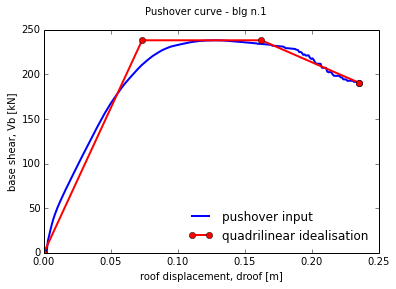
\includegraphics[width=10cm]{./figures/PushoverCurve.png}
\caption{Pushover curve.}
\label{fig:expPushover}
\end{figure}

\begin{figure}[!htbp]
\centering
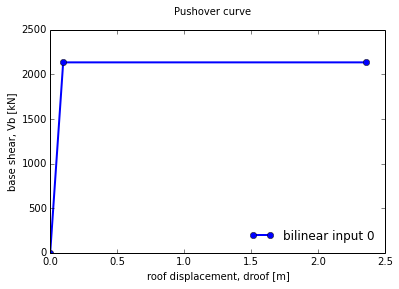
\includegraphics[width=10cm]{./figures/IdealisedCurve.png}
\caption{Idealised pushover curve.}
\label{fig:expIdealised}
\end{figure}

\item Type of output: either fragility curve (probability of exceedance of a set of limit states vs seismic intensity, as shown in Figure \ref{fig:expFragility}) or vulnerability curve (loss ratio vs seismic intensity, as shown in Figure \ref{fig:expVulnerability}).
\end{itemize}

\begin{figure}[!htbp]
\centering
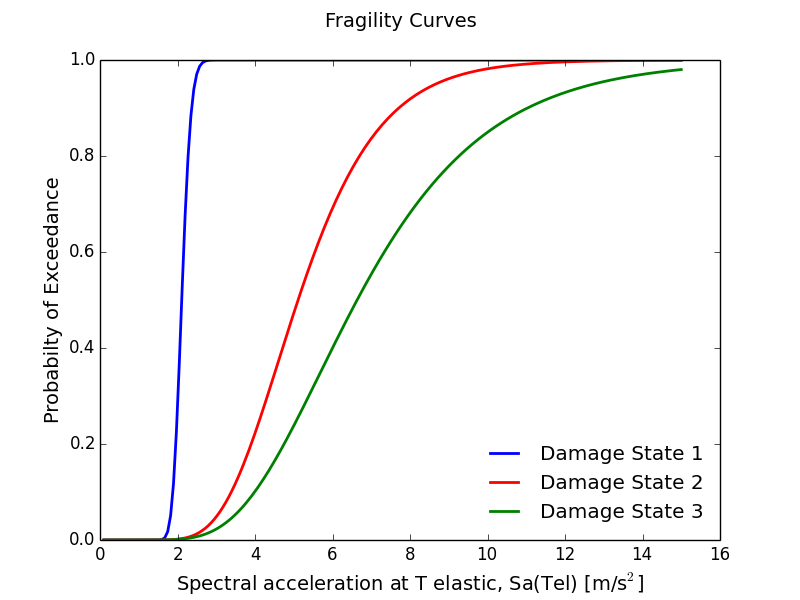
\includegraphics[width=10cm]{./figures/fragility.png}
\caption{Output: fragility curve}
\label{fig:expFragility}
\end{figure}

\begin{figure}[!htbp]
\centering
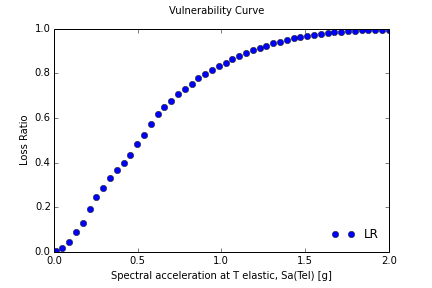
\includegraphics[width=10cm]{./figures/vulnerability.png}
\caption{Output: vulnerability curve}
\label{fig:expVulnerability}
\end{figure}

The outputs are available in the \textit{outputs} folder, located in the \textit{vulnerability} directory. The nonlinear static procedures with dispersion produces results in terms of spectral acceleration in units of g.\\
These options and others need to be defined in the initial section of the script "Define Options". In section \ref{subsubsec:options} the alternatives values that the initial variables can assume and their meaning are described in detail, while the parameters to be inserted in the input files are listed below. They are fully described in section \ref{subsec:nls-ruiz-garcia-miranda} section \ref{subsec:nls-spo2ida} and section  \ref{subsec:nls-dolsek-fajfar}, within the presentation of each procedure.

\subsubsection{Options}
\label{subsubsec:options}
The type of procedure to be performed and the type of inputs at disposal, are set with the variables \textit{an\_type} and \textit{in\_type} respectively. With the variable \textit{an\_type} the user can choose between:

\begin{Verbatim}[frame=single, commandchars=\\\{\}, samepage=true]
an\_type = 0 # Cr-based procedure (Ruiz-Garcia and Miranda, 2007)
an\_type = 1 # spo2ida-based procedure (Vamvatsikos and Cornell, 2006)
an\_type = 2 # R-m-T-based procedure (Dolsek and Fajfar, 2004)
\end{Verbatim}

With the variable \textit{in\_type} the user can choose between:

\begin{Verbatim}[frame=single, commandchars=\\\{\}, samepage=true]
in\_type = 0 # idealised pushover curve
in\_type = 1 # raw results from a pushover analysis
\end{Verbatim}

The variable \textit{vuln} instead gives the opportunity to decide the type of outputs, whether to stop the process at the derivation of the fragility curves, or to go all the way up to the vulnerability curve definition, applying damage-to-loss functions.

\begin{Verbatim}[frame=single, commandchars=\\\{\}, samepage=true]
vuln = 0 # derive fragility curves 
vuln = 1 # derive vulnerability curve
\end{Verbatim}

The variable \textit{g} serves the purpose of defining the units that are used. A floating number must be assigned to the gravity acceleration, compatible with the units used for the period of vibration and for the displacements (if the period is expressed in seconds and displacements are in meters, then g = 9.81). The variable \textit{iml} is a numpy array that identifies the intensity measure levels for which loss ratios are computed and provided in the vulnerability curve. The variable \textit{MC} defines the number of Monte Carlo simulations to account for uncertainty in the damage thresholds.

\begin{Verbatim}[frame=single, commandchars=\\\{\}, samepage=true]
g = 9.81
iml = np.linspace(0.1,15,100)
MC = 25
\end{Verbatim}

The variable \textit{plotflag} allows or inhibits the displaying of plots. It is a python list composed of 4 integers, each one controlling a different plot: idealised pushover curve, 16\%-50\%-84\% ida curves, fragility curves and vulnerability curve respectively. Each integer can take as value either zero or one, whether the corresponding graph has to be displayed or not:

\begin{Verbatim}[frame=single, commandchars=\\\{\}, samepage=true]
plotflag = [1, 1, 1, 1] # plot all the graphs
plotflag = [0, 0, 0, 0] # do not plot any graph
\end{Verbatim}

The following variables set some of the characteristics of the plots:

\begin{itemize}
\item \textit{linew}: integer for defining lines width.
\item \textit{fontsize}: fontsize used for labels, graphs etc.
\item \textit{units}: list of 3 strings defining displacements, forces and Spectral acceleration units, as ['[kN]', '[m]', '[m/s$^2$]'], to be displayed on the axes of the plots.
\end{itemize}

The last set of variables is needed for R-$\mu$-T-based procedure only:
\begin{itemize}
\item \textit{Tc}: constant accel-constant velocity corner period of a Newmark-Hall type spectrum. Default value is 0.5.
\textit{Td}: constant velocity-constant displacement corner period of a Newmark-Hall type spectrum. Default value is 1.8.
\end{itemize}


		\subsection{C$_R$-based procedure (Ruiz-Garcia and Miranda, 2007)}
		\label{subsec:nls-ruiz-garcia-miranda}
		The aim of this procedure, proposed by Vamvatsikos (2014), is the estimation of the median spectral acceleration value $\hat{S}_{a,ds}$, that brings the structure to the attainment of a set of damage states \textit{ds}, and the corresponding dispersion beta $\beta_{S_a}$, the parameters needed for the mathematical representation of fragility in equation \ref{eq:fragility-definition}. The aim is achieved making use of the work by Ruiz-Garcia and Miranda (2007), where the inelastic displacement demand of bilinear SDoF systems is related to the elastic displacement with a simple relationship.

The C$_R$-based procedure presented herein is applicable to bilinear elasto-plastic capacity curve only, and it is suitable for single building fragility curve estimation, as described in section \ref{subsubsec:single-building}. However the fragility curves derived for single buildings can be combined in a unique fragility curve, which considers also the inter-building uncertainty, as described in the following sections.

\subsubsection{Single Building Fragility and Vulnerability function}
\label{subsubsec:single-building}
This procedure provides a simple relationship between median damage state threshold, expressed in terms of top displacement $\hat{d}_{roof, ds}$, at each damage state threshold \textit{ds}, and the corresponding median elastic Spectral displacement value $\hat{S}_{d,ds}(T_1)$.

\begin{equation}
\hat{d}_{roof, ds} = C_R \hat{S}_{d, ds}(T_1) \Gamma_1 \Phi_1
\end{equation}

where $\Gamma_1 \Phi_1$ is the first mode participation factor estimated for the first-mode shape normalised by the roof displacement, and C$_R$ is the inelastic displacement ratio (inelastic over elastic spectral displacement), computed by Ruiz-Garcia and Miranda (2007) for nonlinear SDoF systems, which is a function of the first-mode period of vibration and the relative lateral strength of the system R. Therefore the median Spectral acceleration at the fundamental period of vibration $\hat{S}_{a,ds}(T_1)$ turns out to be expressed as a function of the roof displacement according to the following equation:

\begin{equation}
\hat{S}_{a,ds}(T_1) = \frac{4 \pi^2}{\hat{C}_R T^2 \Gamma_1 \Phi_1} \hat{d}_{roof, ds}
\label{eq:Sa_RGM}
\end{equation}

Estimates of $\hat{C}_R$ parameter are provided by Ruiz-Garcia and Miranda (2007), as result of nonlinear regression analysis of three different measures of central tendency computed from 240 ground motions:

\begin{equation}
\hat{C}_R = 1 + \frac{\hat{R} - 1}{79.12 T_1 ^{1.98}}
\label{eq:Cr_RGM}
\end{equation}

where $\hat{R}$ is given by the following equation:

\begin{equation}
\hat{R}_{ds} = max(0.425(1 - c + \sqrt{c^2 + 2c(2 \hat{\mu}_{ds} - 1) + 1}),1)
\label{eq:R_RGM}
\end{equation}

where c = 79.12 T$^{1.98}$, and $\hat{\mu}_{ds}$ is the median ductility level at the damage state threshold of interest.

For what concerns $\beta_{S_a}$, the dispersion of $\hat{S}_{a,ds}$, it can be computed either in a simplified way or with a comprehensive procedure.

In the simplified approach the following relationship between $S_a$ and the median EDP damage threshold $\hat{\theta}$ (Cornell, 2002) is used:

\begin{equation}
\hat{\theta} = a S_a^b
\end{equation}

so that $\beta_{S_a}$ can be easily derived from the dispersion of $\theta$ due to record-to-record variability, $\beta_{\theta d}$, as in the following:

\begin{equation}
\beta_{S_a} = \frac{1}{b} \beta_{\theta d}
\label{eq:betaSa_RGM}
\end{equation}

$\beta_{\theta d}$ can be obtained assuming that top drift $d_{roof}$ and $\theta$ are proportional, and they thus share the same dispersion. Moreover the dispersion of $d_{roof}$ is the same as the dispersion of C$_R$, since they are also proportional. Finally $\beta_{\theta d}$ can be computed with the following equation, which represents Ruiz-Garcia and Miranda's (2007) estimate of C$_R$ dispersion:

\begin{equation}
\sigma_{\ln(C_R)} = \sigma_{\ln(d_{roof})} = \beta_{\theta d} =  1.975 [\frac{1}{5.876} + \frac{1}{11.749 (T + 0.1)}] [1- \exp(-0.739 (R - 1))]
\label{eq:beta_eq_RGM}
\end{equation}

Uncertainty in the damage state can also be accounted for combining the dispersion of $\theta$ due to uncertainty in the damage state with the dispersion due to record-to-record variability, as in the following equation:

\begin{equation}
\beta_{S_a} = \frac{1}{b} \sqrt{\beta_{\theta d}^2 + \beta_{\theta c}^2}
\label{eq:betaStot_RGM}
\end{equation}

In the comprehensive approach the relationship between the 16$^{th}$, 50$^{th}$ and 84$^{th}$ fractiles of $\mu$ and R needs to be drawn, as represented in Figure \ref{fig:Rmu}. This is done by computing $\beta_{\theta d}$ for a discretised number of R with eq. \ref{eq:beta_eq_RGM}, and obtaining from this value the 16$^{th}$ and 84$^{th}$ fractiles of $\mu$ ($\mu_{16\%}$ and $\mu_{84\%}$), according to the Equations \ref{eq:mu16-beta} and \ref{eq:mu84-beta}.

\begin{figure}[!htbp]
\centering
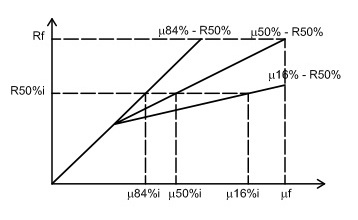
\includegraphics[width=8cm]{./figures/Rmu.jpg}
\caption{R-$\mu$ relationship.}
\label{fig:Rmu}
\end{figure}

\begin{equation}
\mu_{ds,16} = \hat{\mu}_{ds} e^{-\beta_{\theta d,ds}}
\label{eq:mu16-beta}
\end{equation}
\begin{equation}
\mu_{ds,84} = \hat{\mu}_{ds} e^{\beta_{\theta d,ds}}
\label{eq:mu84-beta}
\end{equation}

The median $R_{50\%}$ values have been already computed with eq. \ref{eq:R_RGM}, and $\mu_{16\%}$-$R_{50\%}$, $\mu_{50\%}$-$R_{50\%}$ and $\mu_{84\%}$-$R_{50\%}$ curves can now be drawn.
If uncertainty in the damage criteria $\beta_{\theta c}$ is equal to 0 the $R_{50\%}$, $R_{16\%}$, and $R_{84\%}$ values corresponding to the ductility limit states $\mu_{ds}$ are found interpolating the aforementioned R-$\mu$ curves, and converted into $\hat{S}_{a,ds}$ and $\beta_{S_{a d}}$ according to the following equations:

\begin{equation}
\hat{S}_{a,ds} = R_{50\%}(\mu_{ds}) S_{ay}
\label{eq:SaR}
\end{equation}
\begin{equation}
\beta_{S_{a d}} = \beta_{R(\mu)} = \frac{\ln R(\mu)_{84\%} - \ln R(\mu)_{16\%}}{2}
\label{eq:betaR}
\end{equation} 

where
\begin{equation}
S_{ay} = \frac{4 \pi^2 d_{roof,y}}{T_1^2 g \Gamma_1}
\label{eq:Say}
\end{equation}

If $\beta_{\theta c}$ is different from 0 instead, different values of ductility limit state are sampled from the lognormal distribution with median the median value of the ductility limit state, and dispersion the input $\beta_{\theta c}$.
For each of these ductilities the corresponding $R_{50\%}$, $R_{16\%}$, and $R_{84\%}$ values are found interpolating the aforementioned curves, and converted into $\hat{S}_{a,ds}$ and $\beta_{S_{a d}}$ according to Equations \ref{eq:SaR} and \ref{eq:betaR}.

MC random S$_a$ for each of the MC sampled ductility limit states are computed using $\hat{S}_{a,ds}$ and $\beta_{S_{a d}}$, and their median and dispersion are estimated. These parameters constitute the median $\hat{S}_{a,ds}$ and the total dispersion $\beta_{S_a}$ for the considered damage state. The procedure is repeated for each damage state.

To derive a discrete vulnerability function at certain intensity measure levels, the input damage-to-loss factors are applied to the probability of occurance of each damage state, extracted from the probability of exceedance of each damage state described by the fragility function.
If dispersion due to uncertainty in the limit state is different from zero a vulnerability function is derived for the MC sets of sampled ductility limit states. It results in MC loss ratios (LRs) for each defined intensity measure levels. Finally a lognormal distribution of the loss ratios is assumed at each iml with mean and standard deviation the mean and standard deviation of the all the computed LRs.

\subsubsection{Multiple-Building Fragility and Vulnerability function}
\label{subsubsec:multiple-buildings}
If multiple buildings have been input to derive fragility function for a class of buildings all $\hat{S}_{a, blg}$ and $\beta_{S_a, blg}$ are combined in a single lognormal curve. A minimum of 5 buildings should be considered to obtain reliable results for the class.\\ 
A new issue arises when multiple buildings are considered: the S$_a$ at the fundamental period of each building should be converted to a common intensity measure, to be able to combine the different fragility functions. A common intensity measure is selected to be S$_a$ at the period T$_{av}$, which is a weighted average of the individual building fundamental periods T$_1$. Then each individual fragility needs to be expressed in terms of the common S$_a$(T$_{av}$), using a spectrum. FEMA P-695 far field set of 44 accelerograms (22 records for the two directions) was used to derive a mean uniform hazard spectrum, and the ratio between the S$_a$ at different periods is used to scale the fragility functions. It can be noted that the actual values of the spectrum are not important, but just the spectral shape. 
The median $\hat{S}_a$ is converted to the mean $\mu_{ln(S_a)}$ of the corresponding normal distribution ($\mu_{ln(S_a)} = ln(\hat{S}_a)$) and, simply scaled to the common intensity measure as follows:

\begin{equation}
\mu_{ln(S_a), blg} = \mu_{ln(S_a), blg} S(T_{av})/ S(T_{1, blg})
\end{equation}
\begin{equation}
\beta_{S_a, blg} = \beta_{S_a, blg} S(T_{av})/ S(T_{1, blg})
\label{eq:Sa(Tav)}
\end{equation}

Finally the parameters of the single lognormal curve for the class of buildings, mean and dispersion, can be computed as the weighted mean of the single means and the weighted SRSS of the inter-building and intra-building standard deviation, the standard deviation of the single means and the single dispersions respectively, as shown in the following equations:

\begin{equation}
\mu_{ln(S_a), tot} = \sum_{i=0}^{n.blg} w_{blg-i} \mu_{ln(S_a), blg-i}
\label{eq:combination-lognormals-mu}
\end{equation}
\begin{equation}
\beta_{S_a, tot} = \sqrt{ \sum_{i=0}^{n.blg} w_{blg-i} ((\mu_{ln(S_a), blg-i}-\mu_{ln(S_a), tot})^2+ \beta_{S_a, blg-i}^2})
\label{eq:combination-lognormals-sigma}
\end{equation}

The mean $\mu_{ln(S_a)}$ and total dispersion $\beta_{S_a}$ of the fragility function of the class are converted to logarithmic mean $\mu_{S_a}$ and logarithmic covariance $cov_{S_a}$ (standard deviation $\sigma_{S_a}$ over $\mu_{S_a}$), according to the following equations:

\begin{equation}
\hat{S}_a = e^{\mu_{ln(S_a)}}
\end{equation}
\begin{equation}
\mu_{S_a} = \hat{S}_a e^{\frac{\beta_{S_a}^2}{2}}
\label{eq:median-to-mean}
\end{equation}
\begin{equation}
\sigma_{S_a} = \sqrt[2]{(\beta_{S_a}^2-1) e^{2\ln{ \hat{S}_a}+\beta_{S_a}^2}}
\label{eq:dispersion-to-standard}
\end{equation}
\begin{equation}
cov_{S_a} = \frac{\sigma_{S_a}}{\mu_{S_a} }
\end{equation}

A vulnerability function for a class of buildings can also be obtained, from the single building vulnerability functions. The input damage-to-loss function is applied to the fragility function derived for each building. For the selected intensity measure levels a value of loss ratio $LR_{blg}$ is thus defined for each building. A discrete vulnerability function for the entire class of buildings is represented at each iml by a mean LR, $\mu_{LR,tot}$, equal tot the weighted $LR_{blg}$, and a standard deviation, $\sigma_{LR, tot}$, equal to the weighted standard deviation of all the computed $LR_{blg}$. The $\sigma_{LR, tot}$ of the fragility function of the class is converted to covariance $cov_{LR}$ (standard deviation $\sigma_{LR, tot}$ over $\mu_{LR, tot}$).

\subsubsection{Inputs}
\label{subsubsec:InputCr}
The inputs must be formatted as comma-separated value files (.csv), and saved in the folder \textit{input}, contained in the NSP directory. If any other environment different from Windows is used make sure that the "comma separated values Windows" is selected as saving option when creating the input files. 

If multiple buildings want to be analysed to consider the inter-building uncertainty the parameters relative to each building should be added as additional lines in the input tables, as shown in the examples below, otherwise a single line must be input.

If the user has at disposal an idealised elasto-plastic pushover curve for each building, that is to say that the variable \textit{in\_type} has been set to 0, the following data need to be provided in the corresponding csv files:

\begin{enumerate}
\item First period of vibration T$_1$, corresponding modal participation factor $\Gamma_1$, normalised with respect to the roof displacement, and weight for the combination of different buildings, input in \textit{building\_parameters.csv}, as in the example below:
	\begin{table}[!htbp]
	\centering
	\begin{tabular}{|c|c|c|c|} \hline
	\textbf{n.building} & \textbf{T$_1$} & \textbf{$\Gamma_1$} & \textbf{weights}\\ \hline
	1 & 0.32 & 1.23 & 0.2\\ \hline
	2 & 0.40 & 1.25 & 0.3\\ \hline
	... & ... & ... & ... \\ \hline
	\end{tabular}
	\end{table}
	
\item Roof displacement at each limit state LS and corresponding dispersion $\beta_{\theta c}$ input in \textit{displacement\_profile.csv}, as shown in the example below. If dispersion is unknown, $\beta_{\theta c}$ can be set equal to zero at each LS.
	\begin{table}[!htbp]
	\centering
	\begin{tabular}{|c|c|c|c|} \hline
	\textbf{n.building} & \textbf{LS$_1$} &	\textbf{LS$_2$} &	\textbf{LS$_3$} \\ \hline
	1 & 0.066 & 0.169 & 0.23\\ \hline
	$\beta_{\theta d, 1}$ & 0.1 & 0.3 & 0.4\\ \hline
	2 & 0.08 & 0.172 & 0.25\\ \hline
	$\beta_{\theta d, 2}$ & 0.1 & 0.3 & 0.4\\ \hline	
	\end{tabular}
	\end{table}
	
\item Idealised pushover curve, input in \textit{idealised\_curve.csv} as shown below. The only required parameters are the yielding displacement $d_y$, the ultimate displacement $d_u$ and the yielding force F$_y$.

\begin{table}[!htbp]
\centering
\begin{tabular}{|c|c|c|c|} \hline
\textbf{n.building} & \textbf{d$_y$} & \textbf{d$_u$} & \textbf{F$_y$} \\ \hline
1 & 0.09	& 0.3	 & 523\\ \hline
2 & 0.12	& 0.35	 & 400\\ \hline
... & ...	& ... & ...\\ \hline
\end{tabular}
\end{table}

\item Consequence model (loss ratio per each damage state) consistent with the defined set of damage states, input in \textit{consequence.csv}, as in the example below. A single consequence model can be input. This input is needed only if the variable \textit{vuln} has been set to 1.	
	\begin{table}[!htbp]
	\centering
	\begin{tabular}{|c|c|c|} \hline
	\textbf{DS$_1$} & \textbf{DS$_2$} & \textbf{DS$_3$} \\ \hline
	0.2	& 0.5	 & 1\\ \hline
	\end{tabular}
	\end{table}
	
\end{enumerate}

The user can also decide to input displacements vs base shear at each time step results from a pushover analysis, setting the variable \textit{in\_type} = 0 in the option section. The aforementioned inputs can be used either to derive multilinear idealised curves, setting the option \textit{idealised} = 0, or just to convert the limit states from drift values to roof displacement values without assumptions, and still input an idealised curve, setting the option \textit{idealised} = 1. The following data need to be provided in the corresponding csv files:

\begin{enumerate}
\item T$_1$ and corresponding $\Gamma_1$, weight for the combination of different buildings, number of storeys and height of each storey, input in \textit{building\_parameters.csv}, as in the example below:
	\begin{table}[!htbp]
	\centering
	\begin{tabular}{|c|c|c|c|c|c|c|c|c|} \hline
	\textbf{n.building} & \textbf{T$_1$} & \textbf{$\Gamma_1$} & \textbf{weights} & \textbf{n.Storey} & \textbf{H$_1$} & \textbf{H$_2$} & ... & \textbf{H$_n$} \\ \hline
	1 & 0.32 & 1.23 & 0.2 & 4 & 3 & 3 & ... & 3 \\ \hline
	2 & 0.40 & 1.25 & 0.3 & 4 & 4 & 2.7 & ... & 2.7 \\ \hline
	... & ... & ... & ... & ... & ... & ... & ... & ... \\ \hline
	\end{tabular}
	\end{table}
	
\item Displacements at each storey, at each incremental step of the pushover analysis, input in \textit{displacements\_pushover.csv}, as in the example below: 
	\begin{table}[!htbp]
	\centering
	\begin{tabular}{|c|c|c|c|c|c|c|} \hline
	\textbf{n.building} & \textbf{n.Storey} & \textbf{Step1} & \textbf{Step 2} & \textbf{Storey 3} & ... & \textbf{Step n}\\ \hline
	1 &	1 & 0.0001 &	0.0005 &	0.001 & ... & 0.01\\ \hline
	   &	2 & 0.0003 &	0.0010 &	0.002 & ... & 0.02\\ \hline
	   &	3 & 0.0004 &	0.0016 &	0.003 & ... & 0.03\\ \hline
	   &	4 & 0.0006 &	0.0021 &	0.004 & ... & 0.04\\ \hline
	2 &	1 & 0.0001 &	0.0005 &	0.001 & ... & 0.01\\ \hline
	   &	2 & 0.0005 &	0.0012 &	0.002 & ... & 0.03\\ \hline
	   &	... & ... &	... &	... & ... & ...\\ \hline
	\end{tabular}
	\end{table}
	
\item Base shear at each incremental step of the pushover analysis input in \textit{reactions\_pushover.csv}, as in the example below:
	\begin{table}[!htbp]
	\centering
	\begin{tabular}{|c|c|c|c|c|c|} \hline
	\textbf{n.building} &	\textbf{Step1} & \textbf{Step 2} & \textbf{Storey 3} & ... & \textbf{Step n} \\ \hline
	1 & 0.35 & 0.69 & 1.04 & ... & 29.12\\ \hline
	2 & 0.45 & 0.78 & 2.05 & ... & 40.00\\ \hline
	... & ... & ... & ... & ... & ...\\ \hline
	\end{tabular}
	\end{table}
	
\item Drift limit state and corresponding dispersion $\beta_{\theta c}$ input in \textit{limits.csv}. If dispersion is unknown, $\beta_{\theta c}$ can be set equal to zero at each limit state.
	\begin{table}[!htbp]
	\centering
	\begin{tabular}{|c|c|c|c|} \hline
	\textbf{n.building} & \textbf{LS$_1$} &	\textbf{LS$_2$} &	\textbf{LS$_3$} \\ \hline
	1 & 0.01 &	0.025 & 0.0337\\ \hline
	$\beta_{\theta d, 1}$ &	0.1 & 0.2 & 0.25\\ \hline
	2 & 0.014 &	0.030 & 0.0430\\ \hline
	$\beta_{\theta d, 2}$ &	0.1 & 0.2 & 0.25\\ \hline
	\end{tabular}
	\end{table}

\item Idealised pushover curve, input in \textit{idealised\_curve.csv} if the option \textit{idealised} = 1, as shown below. 
\begin{table}[!htbp]
\centering
\begin{tabular}{|c|c|c|c|} \hline
\textbf{n.building} & \textbf{d$_y$} & \textbf{d$_u$} & \textbf{F$_y$} \\ \hline
1 & 0.09	& 0.3	 & 523\\ \hline
2 & 0.12	& 0.35	 & 400\\ \hline
... & ...	& ... & ...\\ \hline
\end{tabular}
\end{table}

\item Consequence model (loss ratio per each damage state) consistent with the defined set of damage states, input in \textit{consequence.csv}, as in the example below. A single consequence model can be input. This input is needed only if the variable \textit{vuln} has been set to 1.
	\begin{table}[!htbp]
	\centering
	\begin{tabular}{|c|c|c|} \hline
	\textbf{DS$_1$} & \textbf{DS$_2$} & \textbf{DS$_3$} \\ \hline
	0.2	& 0.5	 & 1\\ \hline
	\end{tabular}
	\end{table}
	
\end{enumerate}

\subsubsection{Calculation Steps}
The overall workflow of C$_R$-based procedure is summarised in this section and represented in Figure \ref{fig:Cr_workflow} for the case of a single building fragility/vulnerability function. 

\begin{figure}[!htbp]
\centering
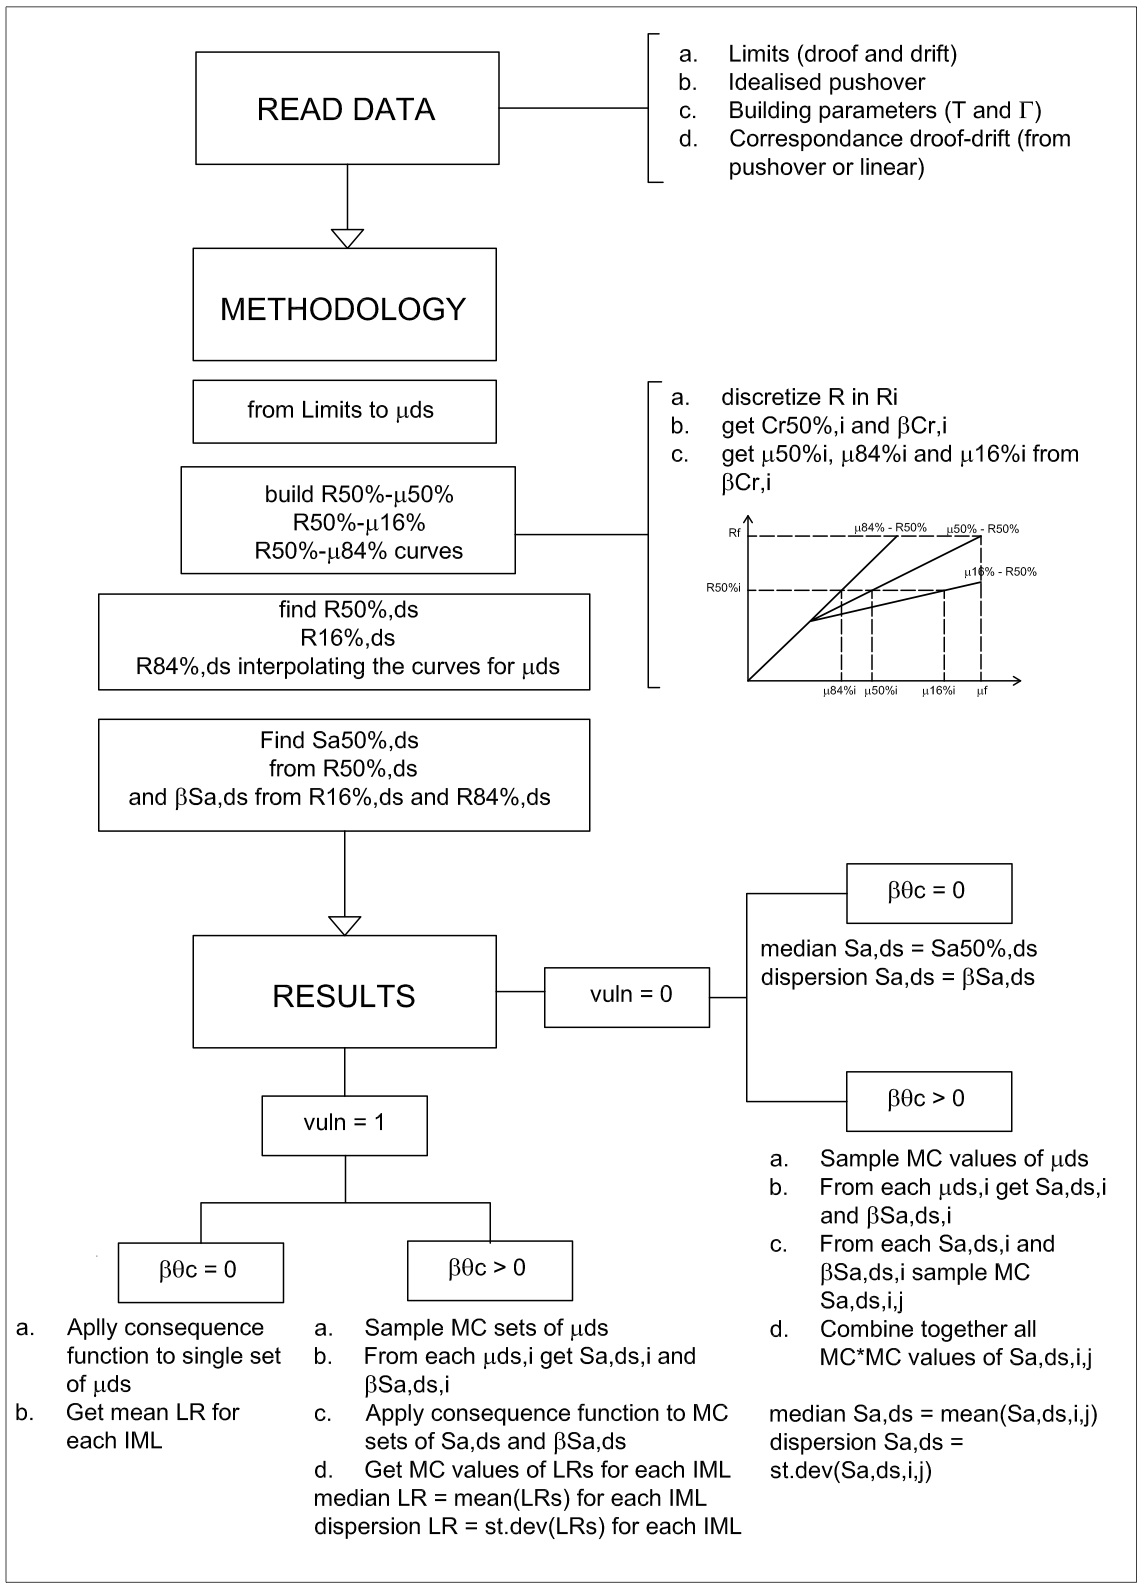
\includegraphics[width=15cm]{./figures/Cr-WorkFlow.jpg}
\caption{C$_R$-based procedure workflow.}
\label{fig:Cr_workflow}
\end{figure}

The option \textit{an\_type} must be set equal to 0 and the option \textit{in\_type} according to the input at disposal. The corresponding inputs should follow the requirements described in section \ref{subsubsec:InputCr}. Given this options the code proceeds with the following steps:\\

\begin{enumerate}
\item \textbf{Process Inputs within \textit{read\_data}  function}\\
\begin{enumerate}
\item If \textit{in\_type} = 0 roof displacement at limit states and idealised pushover are read from \textit{displacement\_profile.csv} and \textit{idealised\_curve.csv} respectively. A one-to-one relationship between roof displacement and drift is assumed.
\item If \textit{in\_type} = 1 results from pushover analysis are extracted from \textit{displacements\_pushover.csv} and \textit{reactions\_pushover.csv}, and drift limit states from \textit{limits.csv}. The relationship between drift and roof displacement is given by the pushover inputs.\\
The idealised 	pushover curve is then derived in the \textit{idealisation} function, where the idealisation process is conducted according to FEMA-440. The elastic stiffness is defined as the 	tangent stiffness passing through the point of the pushover curve where 60\% of the maximum base shear is reached, and the perfectly plastic branch is set at an height equal to 	the maximum base shear. The yielding point is found as the interception between the elastic and the plastic branch.\\
\end{enumerate}

Period, modal participation factor, number of buildings constituting the building class, importance factor (weight) of the each building within the class, average period of the class and $S_a(T_{av})/S_a(T_{blg})$ ratio are also returned by the function \textit{read\_data} .\\

\item \textbf{Fragility curve methodology}\\
The parameters extracted are used in the \textit{simplified\_bilinear} function, within the \textit{fragility\_process} function, to derive ductility levels $\mu_{ds}$, median spectral acceleration $\hat{S}_{a,ds}$ and the total dispersion $\beta_{S_a}$ at each limit state through the following steps:

\begin{enumerate}

\item The idealised MDoF system is transformed into an equivalent SDoF system, using $\Gamma_1$.

\item Ductility levels $\mu_{ds}$ corresponding to each damage threshold, are defined.

\item $\mu_{50\%}$ - $R_{50\%}$, $\mu_{16\%}$ - $R_{50\%}$ and $\mu_{84\%}$ - $R_{50\%}$ relationships are computed, as described in \ref{subsubsec:single-building}.

\item $R_{50\%}$ is computed for the ductility limit states $\mu_{ds}$, interpolating the aforementioned curves, and C$_{R_{50\%}}$ is calculated by mean of equation \ref{eq:Cr_RGM}.

\item $\hat{S}_{a,ds}$ and the corresponding dispersion $\beta_{S_{a d}}$ due to record-to-record variability are computed using eq. \ref{eq:SaR} and \ref{eq:betaR} for each limit state.

\item If dispersion due to uncertainty in the limit state $\beta_{\theta c}$ is different from zero, different ductility limit states are sampled for each median ductility level $\mu_{ds}$. For each sampled ductilities the corresponding $\hat{S}_{a,ds}$ and $\beta_{S_{a d}}$ are found as described in steps (d) and (e), and MC random S$_a$ for each of the MC sampled ductility limit states are computed using $\hat{S}_{a,ds}$ and $\beta_{S_{a d}}$.\\

\end{enumerate}

\item \textbf{Fragility curve results}\\
If number of buildings = 1\\
\begin{enumerate}
\item If \textit{vuln} = 0
the final values of median and dispersion of the fragility curves, $\hat{S}_{a,ds}$ and $\beta_{S_a}$, are computed as the mean and the standard deviation of the MC$^2$ samples of S$_a$, if many $\mu_{ds}$ were sampled at step 2.f, otherwise they correspond to the $\hat{S}_{a,ds}$ and $\beta_{S_{a d}}$, including only record-to-record variability, obtained at step 2.e.
All median values of S$_{a, ds}$ are converted to mean values $\mu_{ln(S_{a, ds})}$; mean $\mu_{ln(S_{a})}$ and total dispersion $\beta_{S_a}$ are then converted to logarithmic mean $\mu_{S_a}$ and logarithmic covariance $cov_{S_a}$, according to equations \ref{eq:median-to-mean} and \ref{eq:dispersion-to-standard} respectively.
Fragility curves for the building are displayed if the variable \textit{plotflag}[2] = 1, and logarithmic $\mu_{S_a}$ and $cov_{S_a}$ are exported in the \textit{outputs} folder.

\item 
If \textit{vuln} =1 if many values were sampled to account for uncertainty in the damage criteria at step 2.f, MC values of loss ratio LRs are defined for the MC sets of $\mu_{ds}$, using the \textit{damage\_to\_loss} function, for each intensity measure level defined in the variable \textit{iml} . Mean and standard deviation of LRs(iml), $\mu_{LR}$ and $\beta_{LR}$, are computed. If $\beta_{\theta c}$= 0 a single set of $\mu_{ds}$ is considered, resulting in no uncertainty in the LR for each iml.
Vulnerability curve for the building is displayed if the variable \textit{plotflag}[3] = 1, and $\mu_{LR}$ and $cov_{LR}$ at each iml are exported in the \textit{outputs} folder.\\

\end{enumerate}

If number of buildings > 1\\
\begin{enumerate}
\item If \textit{vuln} = 0
the final values of median and dispersion of the fragility curves, $\hat{S}_{a,ds}$ and $\beta_{S_a}$, are computed as the mean and the standard deviation of the MC$^2$ samples of S$_a$, if many $\mu_{ds}$ were sampled at step 2.f, otherwise they correspond to the $\hat{S}_{a,ds}$ and $\beta_{S_{a d}}$, including only record-to-record variability, obtained at step 2.e.

All $\hat{S}_{a, ds, blg}(T_1)$ are converted to mean values $\mu_{ln(S_{a, ds, blg})}(T_1)$ and then to the intensity measure in common with the rest of the buildings, $\mu_{ln(S_{a, ds, blg}(T_{av}))}$, according to eq. \ref{eq:Sa(Tav)}.\\
The $\mu_{ln(S_{a, ds, blg}(T_{av}))}$ are finally combined in a single lognormal curve for the building class, as described in section \ref{subsubsec:multiple-buildings}. 

Mean $\mu_{ln(S_{a})}$ and total dispersion $\beta_{S_a}$ are then converted to logarithmic mean $\mu_{S_a}$ and logarithmic covariance $cov_{S_a}$, according to equations \ref{eq:median-to-mean} and \ref{eq:dispersion-to-standard} respectively.

Fragility curves for the class of buildings are displayed if the variable \textit{plotflag}[2] = 1, and logarithmic $\mu_{S_a}$ and $cov_{S_a}$ are exported in the \textit{outputs} folder.

\item 
If \textit{vuln} =1
all $\hat{S}_{a, ds}(T_1)$ for each building are converted to mean $\mu_{ln(S_{a, ds})}(T_1)$ and then to the intensity measure in common with the rest of the buildings, $\mu_{ln(S_{a, ds, blg}(T_{av}))}$, according to eq. \ref{eq:Sa(Tav)}.

if many values were sampled to account for uncertainty in the damage criteria at step 2.f, MC values of loss ratio LRs are defined for the MC sets of $\mu_{ds}$, using the \textit{damage\_to\_loss} function, for each intensity measure level defined in the variable \textit{iml}. Mean and standard deviation of LRs(iml), $\mu_{LR}$ and $\beta_{LR}$, are computed. If $\beta_{\theta c}$= 0 a single set of $\mu_{ds}$ is considered, resulting in no uncertainty in the LR for each iml.
The $\mu_{LR, iml, blg}$ are finally combined in a single mean and standard deviations, as described in section \ref{subsubsec:multiple-buildings}. Vulnerability curve for the class of buildings is displayed if the variable \textit{plotflag}[3] = 1, and $\mu_{LR}$ and $cov_{LR}$ at each iml are exported in the \textit{outputs} folder.

\end{enumerate}

\end{enumerate}


		\subsection{spo2ida-based procedure (Vamvatsikos and Cornell, 2006)}
		\label{subsec:nls-spo2ida}
		The aim of this procedure is the estimation of the median spectral acceleration value $\hat{S}_{a,ds}$, that brings the structure to the attainment of a set of damage states ds, and the corresponding dispersion beta $\beta_{S_a}$, the parameters needed for the mathematical representation of fragility in equation \ref{eq:fragility-definition}. The aim is achieved making use of the tool spo2ida (Vamvatsikos and Cornell, 2006), where static pushover curves are converted into 16\%, 50\% and 84\% ida curves, using empirical relationships from a large database of incremental dynamic analysis results, as shown in Figure~\ref{fig:spo2ida}.

\begin{figure}[!htbp]
\centering
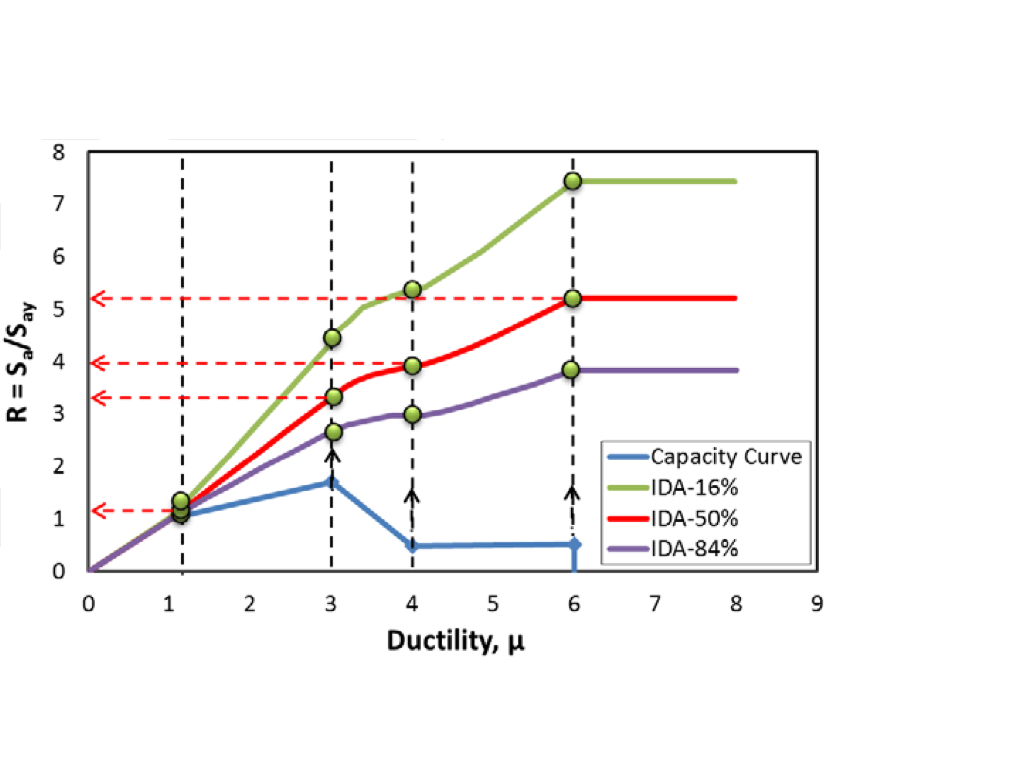
\includegraphics[width=10cm]{./figures/spo2ida.jpg}
\caption{spo2ida tool: IDA curves derived from Pushover curve.}
\label{fig:spo2ida}
\end{figure}

The spo2ida-based procedure presented herein is applicable to any kind of multi-linear capacity curve, and it is suitable for single building fragility curve estimation, as described in section \ref{subsubsec:single-building-spo2ida}. However the fragility curves derived for single buildings can be combined in a unique fragility curve, which considers also the inter-building uncertainty, as described in section \ref{subsubsec:multiple-building-spo2ida}.

\subsubsection{Single-building Fragility and Vulnerability function}
\label{subsubsec:single-building-spo2ida}
Given an idealised capacity curve the spo2ida tool uses an implicit R-$\mu$-T relation to correlate nonlinear displacement, expressed in terms of ductility $\mu$ to the corresponding median capacities in terms of the parameters R. R is the lateral strength ratio, defined as the ratio between the spectral acceleration S$_a$ and the yielding capacity of the system S$_{ay}$. \\

Each branch of the capacity curve, hardening, softening and residual plateau, is converted to a corresponding branch of the three ida curves, using the R-$\mu$-T relation, which is a function of the hardening stiffness, the softening stiffness and the residual force. These parameters are derived from the idealised pushover capacity expressed in $\mu$-R terms, as well as the ductility levels at the onset of each branch. If some of the branches of the pushover curve are missing because of the seismic behaviour of the system, spo2ida can equally work with bilinear, trilinear and quadrilinear idealisations.

The result of the spo2ida routine is thus a list of ductility levels and corresponding R values at 50\%, 16\% and 84\% percentiles. The distribution of R values at each ductility level, due to the record-to-record variability, is assumed to be lognormal and it can be easily converted to the dispersion of S$_a$ using equation \ref{eq:betaR}. 
Median R and its dispersion at ductility levels corresponding to the damage thresholds can thus be determined, and $\hat{S}_{a,ds}$ can be extracted simply multiplying $R_{50\% ds}$ by the yielding capacity of the system $S_{ay}$, as shown in eq. \ref{eq:SaR} and eq. \ref{eq:Say}.\\

If dispersion due to uncertainty in the limit state definition $\beta_{\theta c}$ is different from zero a Monte Carlo sampling needs to be performed to combine it with the record-to-record dispersion. Different values of ductility limit state are sampled from the  lognormal distribution with median the median value of the ductility limit state, and dispersion the input $\beta_{\theta c}$. For each of these ductilities the corresponding median $R_{50\%}$ and R$_{16\%}$, R$_{84\%}$ are found and converted into $\hat{S}_{a,ds}$ and $\beta_S_{a d}$ according to equation \ref{eq:SaR} and \ref{eq:betaR}. MC random S$_a$ for each MC sampled ductility limit state are computed, and their median and the dispersion are estimated. These parameters constitute the median $\hat{S}_{a,ds}$ and the total dispersion $\beta_{S_a}$ for the considered damage state. The procedure is repeated for each damage state.\\

To derive a discrete vulnerability function at certain intensity measure levels, the input damage-to-loss factors are applied to the probability of occurance of each damage state, extracted from the probability of exceedance of each damage state described by the set of fragility curves. 

If dispersion due to uncertainty in the limit state is different from zero a vulnerability function is derived for the MC sets of sampled ductility limit states. It results in MC loss ratios (LRs) for each defined intensity measure levels. Finally a lognormal distribution of the loss ratios is assumed at each iml with mean and standard deviation the mean and the standard deviation of all the computed loss ratios.

\subsubsection{Multiple-Building Fragility and Vulnerability function}
\label{subsubsec:multiple-building-spo2ida}
If multiple buildings have been input to derive a set of fragility curves for a class of buildings all $\hat{S}_{a,blg}$ and $\beta_{S_a,blg}$ are combined in a single lognormal curve for each damage state. A minimum of 5 buildings should be considered to obtain reliable results for the class. The procedure to get $\mu_{S_a,tot}$ and $cov_{S_a,tot}$ for the class of building is the same described in section \ref{subsubsec:multiple-buildings}.

A vulnerability curve for the class of buildings can also be obtained, from the single building vulnerability curves, as described in section \ref{subsubsec:multiple-buildings}.

\subsubsection{Inputs}
\label{subsubsec:InputSpo2ida}
The inputs must be formatted as comma-separated value files (.csv), and saved in the folder \textit{input}, contained in the NSP directory. If any other environment different from Windows is used make sure that the "comma separated values Windows" is selected as saving option when creating the input files. 

If multiple buildings want to be analysed to consider the inter-building uncertainty the parameters relative to each building should be added as additional lines in the tables, as shown in the examples below, otherwise a single line must be input.

If the user has already at disposal an idealised multilinear pushover curve for each building, that is to say that the variable \textit{in\_type} has been set to 0, the following data need to be provided in the corresponding csv files:

\begin{enumerate}
\item First period of vibration $T_1$, corresponding modal participation factor $\Gamma_1$, normalised with respect to the roof displacement, and weight for the combination of different buildings, input in \textit{building\_parameters.csv}, as in section \ref{subsubsec:InputCr}, input n. 1.
	
\item Top displacement at each damage state threshold and corresponding dispersion $\beta_{\theta c}$ input in \textit{displacement\_profile.csv}, as in section \ref{subsubsec:InputCr}, input n. 2. 
	
\item Idealised pushover curve, input in \textit{idealised\_curve.csv} as shown below. The parameters needed to describe the idealised pushover curve are: yielding displacement d$_y$, displacement at the onset of degradation d$_s$, displacement at the onset of residual force d$_{min}$, ultimate displacement d$_u$, maximum force F$_{max}$, residual force F$_{min}$. These parameters are represented in Figure~\ref{fig:quadrilinear}.

\begin{figure}[!htbp]
\centering
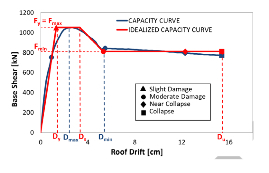
\includegraphics[width=10cm]{./figures/quadrilinear.jpg}
\caption{Idealisation of capacity curve using multilinear elasto-plastic form.}
\label{fig:quadrilinear}
\end{figure}

\begin{table}[!htbp]
\centering
\begin{tabular}{|c|c|c|c|c|c|c|} \hline
\textbf{n.building} & \textbf{d$_y$} & \textbf{d$_s$} & \textbf{d$_{min}$} & \textbf{d$_u$} & \textbf{F$_{max}$} & \textbf{F$_{min}$} \\ \hline
1 & 0.09	& 0.3	& 0.4 & 0.5 & 523 & 430\\ \hline
2 & 0.12	& 0.35	 & 0.43 & 0.5 & 400 & 305\\ \hline	
\end{tabular}
\end{table}

\item Consequence model (loss ratio per each damage state) consistent with the defined set of damage states, input in \textit{consequence.csv}, as in section \ref{subsubsec:InputCr}, input n. 5.
	
\end{enumerate}

If these data are not available, \textit{in\_type} = 0 can be selected and the "raw" results from a pushover analysis can be input instead. The same data as in section \ref{subsubsec:InputCr} for \textit{in\_type} = 0 can be input.

\subsubsection{Calculation Steps}
The overall workflow of spo2ida-based procedure is summarised in this section and represented in Figure \ref{fig:SPO_workflow} for the case of a single building fragility/vulnerability function. 

\begin{figure}[!htbp]
\centering
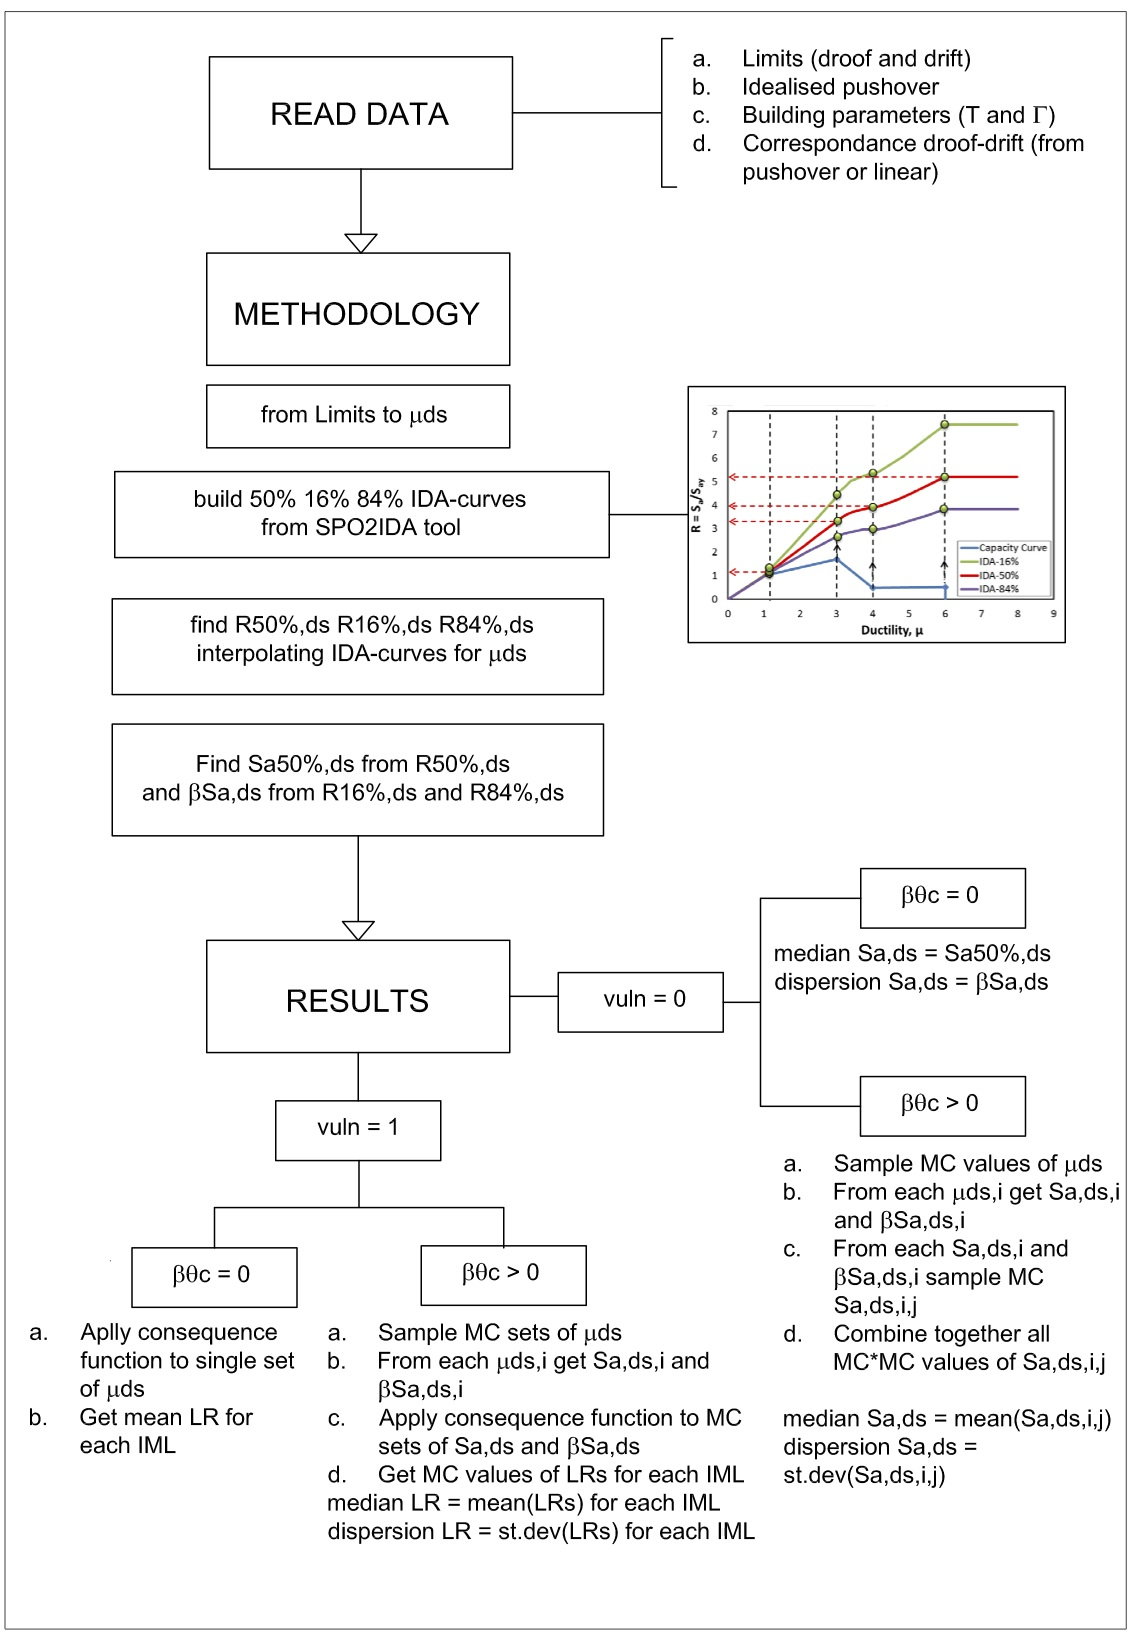
\includegraphics[width=15cm]{./figures/spo-WorkFlow.jpg}
\caption{SPO2IDA-based procedure workflow.}
\label{fig:SPO_workflow}
\end{figure}

The option \textit{an\_type} must be set equal to 1 and the option \textit{in\_type} according to the input at disposal. The corresponding inputs should follow the requirements described in section \ref{subsubsec:InputSpo2ida}. Given these options the code proceeds with the following steps:\\

\begin{enumerate}
\item \textbf{Process Inputs within \textit{read\_data}  function}\\
\begin{enumerate}
\item If \textit{in\_type} = 0, the roof displacement at each limit state and the idealised pushover curve parameters are extracted from \textit{displacement\_profile.csv} and \textit{idealised\_curve.csv} respectively. A one-to-one relationship between roof displacement and drift is assumed.

\item If \textit{in\_type} = 1 the results from a pushover analysis are extracted from \textit{displacements\_pushover.csv} and \textit{reactions\_pushover.csv} and drift limit states from {limits.csv}. The relationship between drift and roof displacement is given by the pushover inputs. The idealised pushover curve is then derived in the \textit{idealisation} function, where the idealisation process is conducted according to the Gem Analytical Vulnerability Guidelines.\\	\end{enumerate}

Period, modal participation factor, number of buildings constituting the building class, importance factor (weight) of the each building within the class, average period of the class and $S_a(T_{av})/S_a(T_{blg})$ ratio are also returned by the function \textit{read\_data} .\\

\item \textbf{Fragility curve methodology}\\
The parameters extracted are used in the \textit{spo2ida\_method} function, within the \textit{fragility\_process} function, to derive ductility levels $\mu_{ds}$, median spectral acceleration $\hat{S}_{a,ds}$ and the total dispersion $\beta_{S_a}$ at each limit state through the following steps:

\begin{enumerate}

\item The idealised MDoF system is transformed into an equivalent SDoF system, using $\Gamma_1$, and the SDoF capacity curve is  expressed in terms of $\mu$-R.

\item Ductility levels $\mu_{ds}$ corresponding to each damage threshold, are defined.

\item The input variables for spo2ida tool are extracted from the capacity curve and they are used as input to get the 16\%-50\%-84\% ida curves.

\item R$_{50\%}$, R$_{16\%}$ and R$_{84\%}$ are computed for the ductility limit states $\mu_{ds}$, interpolating the aforementioned curves.

\item $\hat{S}_{a,ds}$ and the corresponding dispersion $\beta_{S_{a d}}$ due to record-to-record variability are computed using eq. \ref{eq:SaR} and \ref{eq:betaR} for each limit state.

\item If dispersion due to uncertainty in the limit state $\beta_{\theta c}$ is different from zero, different ductility limit states are sampled for each median ductility level $\mu_{ds}$. For each sampled ductilities the corresponding $\hat{S}_{a,ds}$ and $\beta_{S_{a ds}}$ are found as described in steps (d) and (e), and MC random S$_a$ for each of the MC sampled ductility limit states are computed using $\hat{S}_{a,ds}$ and $\beta_{S_{a d}}$.\\

\end{enumerate}

\item \textbf{Fragility curve results}\\
If number of buildings = 1\\
\begin{enumerate}
\item If \textit{vuln} = 0
the final values of median and dispersion of the fragility curves, $\hat{S}_{a,ds}$ and $\beta_{S_a}$, are computed as the mean and the standard deviation of the MC$^2$ samples of S$_a$, if many $\mu_{ds}$ were sampled at step 2.f, otherwise they correspond to the $\hat{S}_{a,ds}$ and $\beta_{S_{a d}}$, including only record-to-record variability, obtained at step 2.e.
All median values of $S_{a, ds}$ are converted to mean values $\mu_{ln(S_{a, ds})}$; mean $\mu_{ln(S_{a})}$ and total dispersion $\beta_{S_a}$ are then converted to logarithmic mean $\mu_{S_a}$ and logarithmic covariance $cov_{S_a}$, according to equations \ref{eq:median-to-mean} and \ref{eq:dispersion-to-standard} respectively.
Fragility curves for the building are displayed if the variable \textit{plotflag}[2] = 1, and logarithmic $\mu_{S_a}$ and $cov_{S_a}$ are exported in the \textit{outputs} folder.

\item 
If \textit{vuln} =1 if many values were sampled to account for uncertainty in the damage criteria at step 2.f, MC values of loss ratio LRs are defined for the MC sets of $\mu_{ds}$, using the \textit{damage\_to\_loss} function, for each intensity measure level defined in the variable \textit{iml}. Mean and standard deviation of LRs(iml), $\mu_{LR}$ and $\beta_{LR}$, are computed. If $\beta_{\theta c}$= 0 a single set of $\mu_{ds}$ is considered, resulting in no uncertainty in the LR for each iml.
Vulnerability curve for the building is displayed if the variable \textit{plotflag}[3] = 1, and $\mu_{LR}$ and $cov_{LR}$ at each iml are exported in the \textit{outputs} folder.\\

\end{enumerate}

If number of buildings > 1\\
\begin{enumerate}
\item If \textit{vuln} = 0
the final values of median and dispersion of the fragility curves, $\hat{S}_{a,ds}$ and $\beta_{S_a}$, are computed as the mean and the standard deviation of the MC$^2$ samples of S$_a$, if many $\mu_{ds}$ were sampled at step 2.f, otherwise they correspond to the $\hat{S}_{a,ds}$ and $\beta_{S_{a d}}$, including only record-to-record variability, obtained at step 2.e.
All $\hat{S}_{a, ds, blg}(T_1)$ are converted to mean values $\mu_{ln(S_{a, ds, blg})}(T_1)$ and then to the intensity measure in common with the rest of the buildings, $\mu_{ln(S_{a, ds, blg}(T_{av}))}$, according to eq. \ref{eq:Sa(Tav)}.\\
The $\mu_{ln(S_{a, ds, blg}(T_{av}))}$ are finally combined in a single lognormal curve for the building class, as described in section \ref{subsubsec:multiple-buildings}. 

Mean $\mu_{ln(S_{a})}$ and total dispersion $\beta_{S_a}$ are then converted to logarithmic mean $\mu_{S_a}$ and logarithmic covariance $cov_{S_a}$, according to equations \ref{eq:median-to-mean} and \ref{eq:dispersion-to-standard} respectively.

Fragility curves for the class of buildings are displayed if the variable \textit{plotflag}[2] = 1, and logarithmic $\mu_{S_a}$ and $cov_{S_a}$ are exported in the \textit{outputs} folder.

\item If \textit{vuln} =1
all $\hat{S}_{a, ds}(T_1)$ for each building are converted to mean $\mu_{ln(S_{a, ds})}(T_1)$ and then to the intensity measure in common with the rest of the buildings, $\mu_{ln(S_{a, ds, blg}(T_{av}))}$, according to eq. \ref{eq:Sa(Tav)}.

if many values were sampled to account for uncertainty in the damage criteria at step 2.f, MC values of loss ratio LRs are defined for the MC sets of $\mu_{ds}$, using the \textit{damage\_to\_loss} function, for each intensity measure level defined in the variable \textit{iml} . Mean and standard deviation of LRs(iml), $\mu_{LR}$ and $\beta_{LR}$, are computed. If $\beta_{\theta c}$= 0 a single set of $\mu_{ds}$ is considered, resulting in no uncertainty in the LR for each iml.
The $\mu_{LR, iml, blg}$ are finally combined in a single mean and standard deviations, as described in section \ref{subsubsec:multiple-buildings}. Vulnerability curve for the class of buildings is displayed if the variable \textit{plotflag}[3] = 1, and $\mu_{LR}$ and $cov_{LR}$ at each iml are exported in the \textit{outputs} folder.

\end{enumerate}

\end{enumerate}


		\subsection{$R-mu-T$-based procedure (Dolsek and Fajfar, 2004)}
		\label{subsec:nls-dolsek-fajfar}
		The aim of this procedure is the estimation of the median spectral acceleration value $\hat{S}_a$, that brings the structure to the attainment of a set of damage states, and the corresponding dispersion beta $\beta_{S_a}$, the parameters needed for the mathematical representation of fragility in equation \ref{eq:fragility-definition}. The aim is achieved making use of a R-$\mu$-T relationship, between reduction factor R, ductility $\mu$ and period T, which is based on the work of Dolsek and Fajfar (2004). The R-$\mu$-T-based procedure presented herein is applicable to any kind of multi-linear capacity curve, and it is suitable for single building fragility curve estimation, as described in section \ref{subsubsec:single-building-DF}. However the fragility curves derived for single buildings can be combined in a unique fragility curve, which considers also the inter-building uncertainty, as described in section \ref{subsubsec:multiple-building-DF}.

\subsubsection{Single Building Fragility and Vulnerability function}
\label{subsubsec:single-building-DF}
This procedure provides a simple relationship between median damage state threshold, expressed in terms of top displacement $\hat{d}_{roof, ds}$, at each damage state threshold \textit{ds}, and the corresponding median elastic Spectral acceleration value $\hat{S}_{a, ds}$, as explained in C$_{R}$-based procedure and reported in the following equation:

\begin{equation}
\hat{S}_{a,ds}(T_1) = \frac{4 \pi^2}{\hat{C}_R T^2 \Gamma_1 \Phi_1} \hat{d}_{roof, ds}
\label{eq:basic_DF}
\end{equation}

The value of C$_R$, the ratio between the inelastic and the elastic spectral displacement, is found from the following equation:

\begin{equation}
\hat{C}_{R} = \frac{\mu_{ds}}{R_{ds}}
\label{eq:Cr_DF}
\end{equation}

where $\mu_{ds}$ and $R_{ds}$ are the median values of ductility level and the reduction factor at the attainment of \textit{ds}. According to the results of an extensive parametric study using three different sets of recorded and semi-artificial ground motions, Dolsek and Fajfar (2004) related the ductility demand $\mu$ and reduction factor R through the following formula:

\begin{equation}
\label{eq:mu_DF}
\mu = \frac{1}{c} (R-R_{0})+\mu_{0}
\end{equation}

In the proposed model $\mu$ is linearly dependent on R within two reduction factor intervals. The parameter c defines the slope of the R–$\mu$ relation, and it depends on the initial period of the system T, the ratio r$_{u}$, the reduction factor R and the corner periods T$_{c}$ and T$_{d}$. T$_{c}$ and T$_{d}$ are the corner periods between the constant acceleration and constant velocity part of the idealised elastic spectrum, and between the constant velocity and constant displacement part of the idealised elastic spectrum respectively. $R_{0}$ and $\mu_{0}$ are the values of R and $\mu$ on the capacity curve corresponding to the hardening behaviour and the softening respectively.

Given the parameters of the multilinear pushover curves (R$_{\mu_{0}}$, $\mu_{0}$, r$_{u}$) and T, the median R - $\mu$ curve can be constructed using the aforementioned relationship. 
The relationship between the 16$^{th}$ and 84$^{th}$ fractiles of $\mu$ and R$_{50}$ needs to be derived using the equations from Ruiz-Garcia and Miranda instead, given that Dolsek and Fajfar do not provide estimates of the dispersion of R. This is done as in the C$_R$-based procedure by computing $\beta_{\theta d}$ for a number of R with eq. \ref{eq:beta_eq_RGM}, and obtaining from this value the 16$^{th}$ and 84$^{th}$ fractiles of $\mu$ ($\mu_{16\%}$ and $\mu_{84\%}$), according to the Equations \ref{eq:mu16-beta} and \ref{eq:mu84-beta}. The $\mu_{50\%}-R_{50\%}$, $\mu_{16\%}-R_50\%$ and $\mu_{84\%}-R_50\%$ curves can thus be drawn.\\

For each $\mu_{ds}$ the corresponding $R_{50\%}$, $R_{16\%}$, and $R_{84\%}$ values are found interpolating the aforementioned curves, and converted into $\hat{S}_{a,ds}$ and $\beta_{S_{a d}}$ according to equations \ref{eq:SaR} and \ref{eq:betaR}.

If dispersion due to uncertainty in the limit state definition $\beta_{\theta c}$ is different from zero it can be combined with the record-to-record dispersion either in a simplified way or with a Monte Carlo sampling procedure.\\

In the simplified method the dispersion of $S_a$ due to uncertainty in the damage state threshold $\beta_{S_{a c}}$ can be found converting the dispersion in the damage threshold $\beta_{\theta c}$, as explaind in section \ref{subsubsec:single-building} and reported in the following equation:

\begin{equation}
\beta_{S_{a c}} = \frac{1}{b} \beta_{\theta c}
\label{eq:betasc_DF}
\end{equation}

In order to derive the b values, which represent the slope of the R-$\mu$ relation in the log-space, a further step needs to be made, because the R-$\mu$-T is suggested by the authors as conservative, since it is not based on the median but on the mean $\mu$ given R. An attempt was made to correct it reducing the median R curve by 15\%, $R_{50\% corrected}$, as shown in equation \ref{eq:Rcorrected}, and extrapolating the corresponding $\mu_{50\% corrected}$.

\begin{equation}
R_{50\% corrected}=0.85 R_{50\%}
\label{eq:Rcorrected}
\end{equation}
\begin{equation}
b = \frac{ln(\mu_{50\% corrected})}{ln(R_{50\% corrected})}
\label{eq:bcorrected_DF}
\end{equation}

Finally the dispersion of $S_a$ due to record-to-record variability, can be combined with the dispersion of $S_a$ due to uncertainty in the damage state threshold, as in the following equation:

\begin{equation}
\beta_{S_a} = \sqrt{\beta_{S_{a c}}^2+\beta_{S_{a d}}^2}
\label{eq:betatot_DF}
\end{equation}

In the Monte Carlo approach different values of ductility limit state are sampled from the lognormal distribution with median the median value of the ductility limit state, and dispersion the input $\beta_{\theta c}$.
For each of these ductilities the corresponding $R_{50\%}$, $R_{16\%}$, and $R_{84\%}$ values are found interpolating the $\mu_{50\%}-R_{50\%}$, $\mu_{16\%}-R_50\%$ and $\mu_{84\%}-R_50\%$ curves, and converted into $\hat{S}_{a,ds}$ and $\beta_{S_{a d}}$ according to Equations \ref{eq:SaR} and \ref{eq:betaR}.

MC random S$_a$ for each of the MC sampled ductility limit states are computed using $\hat{S}_{a,ds}$ and $\beta_{S_{a d}}$, and their median and dispersion are estimated. These parameters constitute the median $\hat{S}_{a,ds}$ and the total dispersion $\beta_{S_a}$ for the considered damage state. The procedure is repeated for each damage state.

To derive a discrete vulnerability function at certain intensity measure levels, the input damage-to-loss factors are applied to the probability of occurance of each damage state, extracted from the probability of exceedance of each damage state described by the fragility function.
If dispersion due to uncertainty in the limit state is different from zero a vulnerability function is derived for the MC sets of sampled ductility limit states. It results in MC loss ratios for each defined intensity measure levels. Finally a lognormal distribution of the loss ratios is assumed at each iml with mean and standard deviation the mean and standard deviation of the all the computed LRs.

\subsubsection{Multiple Building Fragility and Vulnerability function}
\label{subsubsec:multiple-building-DF}
 If multiple buildings have been input to derive fragility function for a class of buildings all $\hat{S}_{a, blg}$ and $\beta_{S_a, blg}$ are combined in a single lognormal curve as described in section \ref{subsubsec:multiple-buildings}. The same holds for vulnerability function, as described in the same section.

\subsubsection{Inputs}
The data the user needs provided and the their format is described in section \ref{subsubsec:InputSpo2ida}

\subsubsection{Calculation Steps} 
The overall workflow of R-$\mu$-T-based procedure is summarised in this section and represented in Figure \ref{fig:Cr_workflow} for the case of a single building fragility/vulnerability function. 

\begin{figure}[!htbp]
\centering
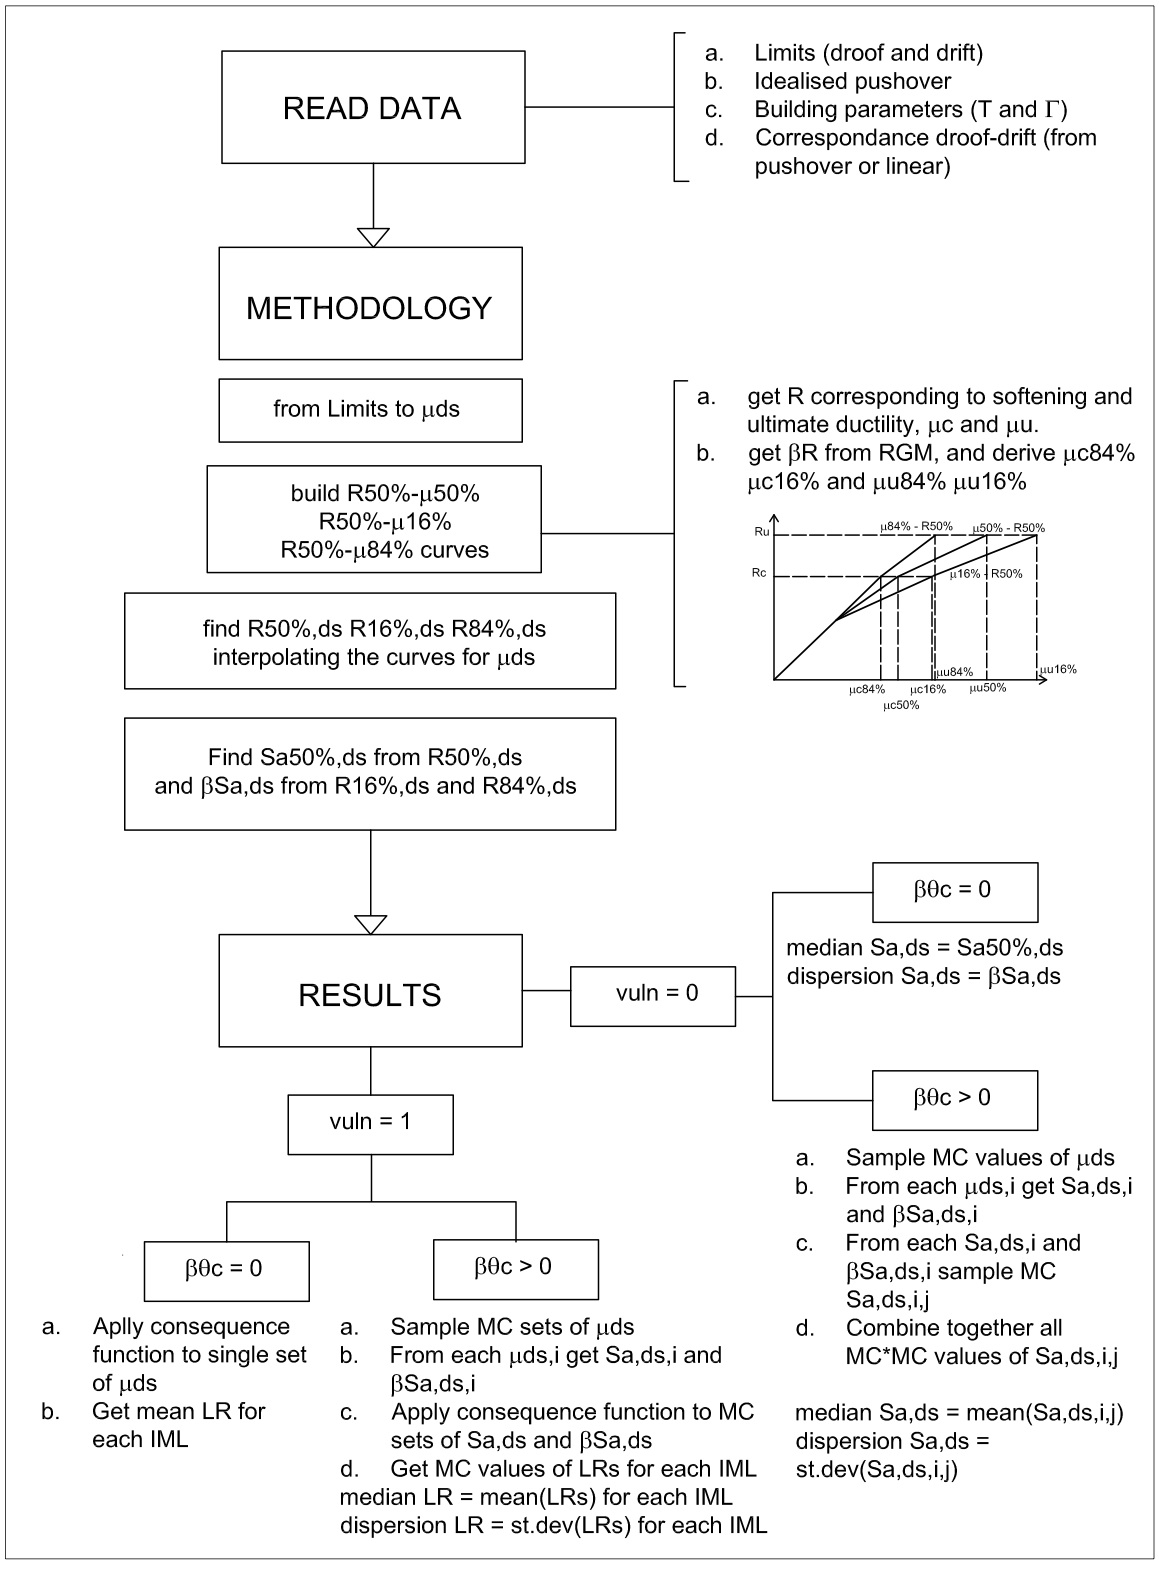
\includegraphics[width=15cm]{./figures/DF_WorkFlow.jpg}
\caption{R-$\mu$-T-based procedure workflow.}
\label{fig:Cr_workflow}
\end{figure}

The option \textit{an\_type} must be set equal to 2 and the option \textit{in\_type} according to the input at disposal. The corresponding inputs should follow the requirements described in section \ref{subsubsec:InputSpo2ida}.Given these options the code proceeds with the following steps:\\

\begin{enumerate}
\item \textbf{Process Inputs within \textit{read\_data}  function}\\

\begin{enumerate}
\item If \textit{in\_type} = 0, the roof displacement at each limit state and the idealised pushover curve parameters are extracted from \textit{displacement\_profile.csv} and \textit{idealised\_curve.csv} respectively. A one-to-one relationship between roof displacement and drift is assumed
\item If \textit{in\_type} = 1 the results from a pushover analysis are extracted from \textit{displacements\_pushover.csv} and \textit{reactions\_pushover.csv} and drift limit states from {limits.csv}. The relationship between roof displacement and drift is given by the pushover inputs. The idealised pushover curve is then derived in the \textit{idealisation} function, where the idealisation process is conducted according to the Gem Analytical Vulnerability Guidelines.\\
\end{enumerate}

Period, modal participation factor, number of buildings constituting the building class, importance factor (weight) of the each building within the class, average period of the class and $S_a(T_{av})/S_a(T_{blg})$ ratio are also returned by the function \textit{read\_data} .\\

\item \textbf{Fragility curve methodology}\\
The parameters extracted are used in the \textit{DF\-fragility} function, within the \textit{fragility\_process} function, to derive ductility levels $\mu_{ds}$, median spectral acceleration $\hat{S}_{a,ds}$ and the total dispersion $\beta_{S_a}$ at each limit state through the following steps:

\begin{enumerate}

\item The idealised MDoF system is transformed into an equivalent SDoF system, using $\Gamma_1$, and the SDoF capacity curve is expressed in terms of $\mu$ and R.

\item Ductility levels $\mu_{ds}$ corresponding to each damage threshold, are defined.

\item The input variables R$_{\mu_{0}}$, $\mu_{0}$, r$_{u}$ for Equation \ref{eq:mu_DF} are inferred from the capacity curve and median $\mu$ - R relationship is computed using Equation \ref{eq:mu_DF}.

\item $\mu_{16\%}$ - $R_{50\%}$ and $\mu_{84\%}$ - $R_{50\%}$ relationships are computed as in C$_R$-based procedure.

\item $R_{50\%}$, $R_{16\%}$ and $R_{84\%}$ is computed for the ductility limit states $\mu_{ds}$, interpolating the aforementioned R - $\mu$ curves.

\item $\hat{S}_{a,ds}$ and the corresponding dispersion $\beta_{S_{a d}}$ due to record-to-record variability are computed using eq. \ref{eq:SaR} and \ref{eq:betaR} for each limit state.

\item If dispersion due to uncertainty in the limit state $\beta_{\theta c}$ is different from zero, different ductility limit states are sampled for each median ductility level $\mu_{ds}$. For each sampled ductilities the corresponding $\hat{S}_{a,ds}$ and $\beta_{S_{a ds}}$ are found as described in steps from (d) to (f), and MC random S$_a$ for each of the MC sampled ductility limit states are computed using $\hat{S}_{a,ds}$ and $\beta_{S_{a d}}$.\\

\end{enumerate}

\item \textbf{Fragility curve results}\\
If number of buildings = 1\\
\begin{enumerate}
\item If \textit{vuln} = 0
the final values of median and dispersion of the fragility curves, $\hat{S}_{a,ds}$ and $\beta_{S_a}$, are computed as the mean and the standard deviation of the MC$^2$ samples of S$_a$, if many $\mu_{ds}$ were sampled at step 2.g, otherwise they correspond to the $\hat{S}_{a,ds}$ and $\beta_{S_{a d}}$, including only record-to-record variability, obtained at step 2.f.

All median values of $S_{a, ds}$ are converted to mean values $\mu_{ln(S_{a, ds})}$; mean $\mu_{ln(S_{a})}$ and total dispersion $\beta_{S_a}$ are then converted to logarithmic mean $\mu_{S_a}$ and logarithmic covariance $cov_{S_a}$, according to equations \ref{eq:median-to-mean} and \ref{eq:dispersion-to-standard} respectively.

Fragility curves for the building are displayed if the variable \textit{plotflag}[2] = 1, and logarithmic $\mu_{S_a}$ and $cov_{S_a}$ are exported in the \textit{outputs} folder.

\item 
If \textit{vuln} =1
if many values were sampled to account for uncertainty in the damage criteria at step 2.f, MC values of loss ratio LRs are defined for the MC sets of $\mu_{ds}$, using the \textit{damage\_to\_loss} function, for each intensity measure level defined in the variable \textit{iml}. Mean and standard deviation of LRs(iml), $\mu_{LR}$ and $\beta_{LR}$, are computed. If $\beta_{\theta c}$= 0 a single set of $\mu_{ds}$ is considered, resulting in no uncertainty in the LR for each iml.
Vulnerability curve for the building is displayed if the variable \textit{plotflag}[3] = 1, and $\mu_{LR}$ and $cov_{LR}$ at each iml are exported in the \textit{outputs} folder.\\

\end{enumerate}

If number of buildings > 1\\
\begin{enumerate}
\item If \textit{vuln} = 0
the final values of median and dispersion of the fragility curves, $\hat{S}_{a,ds}$ and $\beta_{S_a}$, are computed as the mean and the standard deviation of the MC$^2$ samples of S$_a$, if many $\mu_{ds}$ were sampled at step 2.g, otherwise they correspond to the $\hat{S}_{a,ds}$ and $\beta_{S_{a d}}$, including only record-to-record variability, obtained at step 2.f.

All $\hat{S}_{a, ds, blg}(T_1)$ are converted to mean $\mu_{ln(S_{a, ds, blg})}(T_1)$ and then to the intensity measure in common with the rest of the buildings, $\mu_{ln(S_{a, ds, blg}(T_{av}))}$, according to eq. \ref{eq:Sa(Tav)}.\\
The $\mu_{ln(S_{a, ds, blg}(T_{av}))}$ are finally combined in a single lognormal curve for the building class, as described in section \ref{subsubsec:multiple-buildings}. 

Mean $\mu_{ln(S_{a})}$ and total dispersion $\beta_{S_a}$ are then converted to logarithmic mean $\mu_{S_a}$ and logarithmic covariance $cov_{S_a}$, according to equations \ref{eq:median-to-mean} and \ref{eq:dispersion-to-standard} respectively.

Fragility curves for the class of buildings are displayed if the variable \textit{plotflag}[2] = 1, and logarithmic $\mu_{S_a}$ and $cov_{S_a}$ are exported in the \textit{outputs} folder.

\item 
If \textit{vuln} =1
all $\hat{S}_{a, ds}(T_1)$ for each building are converted to mean $\mu_{ln(S_{a, ds})}(T_1)$ and then to the intensity measure in common with the rest of the buildings, $\mu_{ln(S_{a, ds, blg}(T_{av}))}$, according to eq. \ref{eq:Sa(Tav)}.

For each intensity measure level defined in the variable \textit{iml} MC values of loss ratio LRs are defined for the MC sets of $\mu_{ds}$, if many values were sampled to account for uncertainty in the damage criteria at step 2.f, using the \textit{damage\_to\_loss} function. Mean and standard deviation of LRs(iml), $\mu_{LR}$ and $\beta_{LR}$, are computed. If $\beta_{\theta c}$= 0 a single set of $\mu_{ds}$ is considered, resulting in no uncertainty in the LR for each iml.\\

The $\mu_{LR, iml, blg}$ are finally combined in a single mean and standard deviations, as described in section \ref{subsubsec:multiple-buildings}. Vulnerability curve for the class of buildings is displayed if the variable \textit{plotflag}[3] = 1, and $\mu_{LR}$ and $cov_{LR}$ at each iml are exported in the \textit{outputs} folder.

\end{enumerate}

\end{enumerate}



		\subsection{NLS methods without record-to-record dispersion}
		\label{subsec:nls-no-dispersion}
		Still to implement

	\section{Non-linear Dynamic (NLD) Methods}
	\label{sec:nld-intro}
	Nonlinear Dynamic Methods are based on the results of many dynamic analyses, which relate the seismic response of a structure, represented by an Engineering Demand Parameter (EDP), like maximum top displacement, maximum inter-storey drift ratio, maximum top drift etc., to the Intensity Measure Level (IML) of the input accelerograms. 
Many methods exists in literature to perform a series of dynamic analysis and to post-process the results in order to derive fragility curves. Some of them treat a single building to estimate directly the median seismic intensity value corresponding to the attainment of different damage state thresholds (limit states), and the corresponding dispersion (Vamvatsikos and Cornell, 2002, Ellingwood and Kinali, 2009). Others treat a class of buildings, and lead to the evaluation of the probabilities of different damage states for a series of IMLs and thus to the set up of a damage probability matrix (Singhal and Kiremidjian, 1996, Silva et al., 2013).

The former approach has been implemented in the Ida-based procedure and explained in section \ref{subsec:nld-ida}, the latter in the DPM-based procedure, explained in section \ref{subsec:nld-dpm}. Both sections contains the necessary scientific background behind the code and their step-by-step implementation in the python script.

		\subsection{Using the NLD module}
		\label{subsec:nld-how-to-use}
		To start using the nonlinear dynamic method a command line text editor should be used to enter manually the folder location where the \textit{rmtk} has been saved, as shown in the example below:

\begin{Verbatim}[frame=single, commandchars=\\\{\}, samepage=true]
cd path/to/rmtk/folder/rmtk/vulnerability
\end{Verbatim}

Where /path/to/rmtk/folder/ is the system path to the location of the \textit{rmtk} folder. From the text editor iPython browser page can be opened with the following command line:

\begin{Verbatim}[frame=single, commandchars=\\\{\}, samepage=true]
ipython-2.7 notebook --pylab=inline
\end{Verbatim}

Once the iPython page is opened on the browser, the python scripts contained in the \textit{rmtk} directory will be visible. The file \textit{NDM.ipynb} should be selected to start the calculations.

In the initial section of the script "Define Options" the user needs to set the options and to enter the input corresponding to the defined options in the folder \textit{NDP/input}. In section~\ref{subsubsec:NDMoptions} the alternatives values that the initial variables can assume and their meaning are described in detail, while the parameters to be inserted in the input files are fully described in section~\ref{subsubsec:NDMinputs}.

		\subsection{Damage probability matrix DPM-based procedure}
		\label{subsec:nld-dpm}
		This procedure performs the post-processing part of a set of dynamic analyses to first assemble a damage probability matrix, and then use this data for the derivation of a fragility function. Therefore the results of a set of dynamic analyses previously run have to be input to start the process. A list of intensity measure associated to each accelerogram, and corresponding EDP for each structure of the building class can be input, along with the set of limit states expressed in terms of the same EDP. The EDPs resulting from the dynamic analyses are compared with the limit state displacements and a global damage state is assigned to each structure. Thus, for each record, the number of frames in each damage state can be obtained. The distribution of buildings in each damage state is organised in the damage probability matrix, with a number of rows equal to the number of ground motion records and a number of columns equal to the number of damage states.

The processing of the data continue with the estimation of the cumulative fraction of structures in each damage state, summing the percentages of frames belonging to all the subsequent damage states. A lognormal cumulative distribution function, expressing the probability of exceeding each damage state in a continuous fashion, is then fit to these results, leading to the statistical parameters of the fragility curves. The regression analysis is carried out using the maximum likelihood method.

This function have the advantage of accounting for the record-to-record variability by the use of many ground motion records, and the inter-building variability subjecting to the same set of accelerograms hundreds of structures representing the entire building class.

To derive a discrete vulnerability function at certain intensity measure levels, the input damage-to-loss factors are applied to the probability of occurance of each damage state, extracted from the probability of exceedance of each damage state described by the fragility function. For the vector of selected intensity measure levels a value of loss ratio is thus defined.

\subsubsection{Options}
\label{subsubsec:NDMoptions}
In the Options the user has to define first of all the type of inputs at disposal, setting the variable \textit{in\_ type}, choosing between entering a damage count matrix, which corresponds to a damage probability matrix, where the probabilities of each damage state are substituted by the count of buildings in that damage state, or IML and corresponding EDPs for each dynamic analysis

\begin{Verbatim}[frame=single, commandchars=\\\{\}, samepage=true]
in\_type = 0 # damage count matrix 
in\_type = 1# IMLs and EDPs 
\end{Verbatim}

The variable \textit{vuln} instead gives the opportunity to decide the type of outputs, whether to stop the process at the derivation of the fragility curves, or to go all the way up to the vulnerability curve definition, applying damage-to-loss functions.

\begin{Verbatim}[frame=single, commandchars=\\\{\}, samepage=true]
vuln = 0 # derive fragility curves 
vuln = 1 # derive vulnerability curve
\end{Verbatim}

The variable g has to be set to the value of the gravity acceleration, expressed consistently with the units used for the intensity measure input data. For example if the intensity measure used is PGA expressed in g, the variable g will be set to 1, if PGA is expressed in m/s$^2$ instead g will be set to 9.81.

The variable \textit{iml} is a numpy array that identifies the intensity measure levels for which loss ratios are computed and provided in the vulnerability curve.

\begin{Verbatim}[frame=single, commandchars=\\\{\}, samepage=true]
iml = np.linspace(0.1,15,100)
\end{Verbatim}

The variable \textit{plotflag} allows or inhibits the displaying of plots. It is a python list composed of 2 integers, each one controlling a different plot: fragility and vulnerability function respectively. Each integer can take as value either zero or one, whether the corresponding graph has to be displayed or not:

\begin{Verbatim}[frame=single, commandchars=\\\{\}, samepage=true]
plotflag = [1, 1] # plot all the graphs
plotflag = [0, 0] # do not plot any graph
\end{Verbatim}

The following variables set some of the characteristics of the plots:
\begin{itemize}
\item IMlabel: list of one strings defining the IM on the x axis as ['Sa(Tel)-m/s$^{2}$']
\item linew: integer for defining lines width.
\item fontsize : fontsize used for labels, graphs etc.
\end{itemize}

\subsubsection{Inputs}
\label{subsubsec:NDMinputs}
The inputs must be formatted as comma-separated value files (.csv), and saved in the folder \textit{input}, contained in the NDP directory. If any other environment different from Windows is used make sure that the "comma separated values Windows" is selected as saving option when creating the input files.  

Two types of input can be entered, whether the results of the set of dynamic analyses performed have already been organised in a damage probability matrix for or not. In the former case the variable \textit{in\_type} should be set to 0 and the damage count matrix should be input in the csv file \textit{dcm.csv}. The first two columns refer to the number of record and the corresponding intensity measure level, the following columns report the number of buildings in each damage state, as shown in the following table:

\begin{table}[!htbp]
\centering
\begin{tabular}{|c|c|c|c|c|} \hline
\textbf{n.records} & \textbf{Intensity Measure Level} & \textbf{DS$_0$} & \textbf{DS$_1$} & \textbf{DS$_2$} \\ \hline
1 & 49.852 &	30 &	16 &	54\\ \hline
2 & 47.056 &	54 &	15 &	31\\ \hline
3 & 33.012 &	59 &	10 &	31\\ \hline
4 & 82.125 &	24 &	26 &	50\\ \hline
... & ... & ... & ... & ... \\ \hline
5 & 37.499 &	58 &	5 &	37\\ \hline
\end{tabular}
\end{table}

In the latter case the variable \textit{in\_type} should be set to 1, and the results of the set of dynamic analyses should be entered in the \textit{edp.csv} file in the following fashion: number of record, corresponding IML, and corresponding EDPs for each building subjected to that record.

\begin{table}[!htbp]
\centering
\begin{tabular}{|c|c|c|c|c|c|} \hline
\textbf{n.records} & \textbf{IML} & \textbf{edp$_{blg,1}$} & \textbf{edp$_{blg,2}$} & \textbf{...} & \textbf{edp$_{blg,n}$} \\ \hline
1 &	69.209 &	-0.00069 &	0.00031 & ... &	0.00131\\ \hline
2 &	75.470 &	0.00102 & 	0.00202 & ... &	0.00302\\ \hline
3 &	62.233 &	-0.00090 &	0.00010 & ... &	0.00110\\ \hline
4 &	168.47 &	-0.00246 &	-0.00146 & ... &	-0.00046\\ \hline
5 &	67.612 &	0.00095 & 	0.00195 & ... &	0.00295\\ \hline
... & ... & ... & ... & ... & ...\\ \hline
n &	34.484 &	0.00036 & 	0.00136 & ... & 	0.00236\\ \hline
\end{tabular}
\end{table}

In this case also the limit states must be input in the \textit{limits.csv} file. Each line of the file corresponds to the limit states of a building, but if all the buildings share the same limits a single line can be input.

\begin{table}[!htbp]
\centering
\begin{tabular}{|c|c|c|c|c|} \hline
\textbf{n.building} & \textbf{LS$_1$} & \textbf{LS$_2$} & \textbf{LS$_3$} & \textbf{LS$_4$} \\ \hline
1 & 0.003 &	0.010 &	0.025 &	0.0337\\ \hline
2 & 0.004 &	0.015 &	0.020 &	0.035\\ \hline
3 & 0.002 &	0.019 &	0.027 &	0.032\\ \hline
... & ... & ... & ... & ...\\ \hline
n & 0.0024 &	0.016 &	0.025 &	0.03\\ \hline
\end{tabular}
\end{table}

\subsubsection{Calculations}
The overall workflow of the DPM-based procedure is summarised in this section. The option \textit{in\_type} should be set according to the input at disposal. The corresponding inputs should follow the requirements described in the previous section. At this point the code proceeds with the following steps:

\begin{enumerate}
\item In the function \textit{read\_data} the inputs are read and the damage count matrix is returned.
\begin{enumerate}
\item If \textit{in\_type} = 0, the damage count matrix is extracted directly from the \textit{dcm.csv} file.

\item If \textit{in\_type} = 1 the IMLs of the records used in the dynamic analyses and the corresponding EDPs are extracted from \textit{edp.csv} and the limit states for each building, expressed in terms of the same EDP, are extracted from \textit{limits.csv}.	 These data are converted into a damage count matrix according to the method described in section \ref{subsec:nld-dpm}.
\end{enumerate}

\item The parameters extracted are used to derive the Probability of Exceedance (PoE) of each limit state for each IML, as described in section \ref{subsec:nld-dpm}.

\item The PoEs are fitted with a lognormal function using the maximum likelihood method. The mean $\mu_{ln IML}$ and standard deviation $\sigma_{ln IML}$ of the corresponding normal distribution for the entire class of buildings are found for each limit state.

\item The $\mu_{ln IML}$ and $\sigma_{ln IML}$ are converted to logarithmic $\mu_{IML}$ and $\sigma_{IML}$. The fragility curves for the class of buildings are displayed if the variable \textit{plotflag}[0] = 1, and the logarithmic $\mu_{IML}$ and $\sigma_{IML}$ are exported in the \textit{outputs} folder.

\item If \textit{vuln} =1:  For the intensity measure levels defined in the variable \textit{iml} a value of loss ratio is defined, according to section \ref{subsec:nld-dpm}. A vulnerability curve for the class of buildings is displayed if the variable~\textit{plotflag}[1] = 1, and the loss ratios at each iml are exported in the \textit{outputs} folder.

\end{enumerate}

		\subsection{Post-processing IDA}
		\label{subsec:nld-ida}
		Post processing IDA

		% \subsection{Multiple stripe analysis (Jalayer, 2003)}
		% \label{subsec:nld-msa}
		% \input{./tex/nld-msa}